\documentclass[12pt,a4paper]{ctexart}

\usepackage{ctex}
\usepackage[top=2.5cm,bottom=2.5cm,left=2.8cm,right=2.8cm]{geometry}
\usepackage{amsmath,amssymb,amsfonts}
\usepackage{algorithm}
\usepackage{algorithmicx}
\usepackage{algpseudocode}
\usepackage{bm}
\usepackage{graphicx}
\usepackage{booktabs}
\usepackage{multirow}
\usepackage{subcaption}
\usepackage{float}
\usepackage[colorlinks=true,linkcolor=blue,citecolor=blue,urlcolor=blue]{hyperref}
\usepackage[super,square,sort&compress,comma]{natbib}
\usepackage{url}
\usepackage{enumitem}
\usepackage{color}
\usepackage{xcolor}
\usepackage{textcomp}
\usepackage{diagbox}

\graphicspath{{figures/}}

\title{\textbf{基于 DreamerV3 世界模型的居家服务机器人导航系统研究}}
\author{陈杉杉}
\date{\today}

\begin{document}

\maketitle

\begin{abstract}
随着全球人口老龄化程度的持续加深，居家养老服务和辅助生活技术的发展日益受到社会各界的重视。
服务机器人作为缓解养老护理人力资源短缺、提升老年人独立生活能力的关键技术载体，正加速从实验室研究走向家庭实际部署。
在复杂多变的居家环境中实现高效且鲁棒的自主导航，是服务机器人走向真正实用化必须首先攻克的核心技术瓶颈之一。

传统机器人导航方案普遍采用基于地图的模块化架构，典型技术栈包括同时定位与建图（SLAM）、全局路径规划、局部轨迹优化以及底层运动控制等多个独立子模块。
此类模块串联架构在实际部署中暴露出若干结构性问题：各模块独立设计且独立优化，缺乏统一的全局优化目标，导致感知与控制误差在模块间逐级累积；模块间的接口适配和参数联调耗时费力，系统对陌生环境的迁移适应性显著不足；更为关键的是，传统架构本质上是一种被动响应式决策模式，无法对未来的环境状态演化进行前瞻性推演，因而在需要长程规划的复杂任务中表现严重受限。

近年来，以 Dreamer 系列为代表的基于世界模型的强化学习方法取得了突破性进展。
其核心思想在于，智能体不仅学习执行策略，还同步学习一个能够预测环境未来状态的世界模型，并利用该模型在紧凑的潜在空间中展开想象规划，实现对不同候选动作序列预期后果的前瞻性评估。

本文基于 DreamerV3 算法框架，面向居家服务机器人导航场景，构建了从 RGB 视觉观测到离散动作决策的端到端学习系统。
在自主设计的 HomeNav-v0 居家仿真环境中，部署了包含约 1049 万参数的循环状态空间模型（RSSM）并进行系统训练与评估。
实验结果表明，经过 500,000 步训练后，智能体的策略得分从初始约 $-10$ 提升至约 $+15$，任务完成效率提升约 10 倍（单回合步数从约 200 步缩短至约 20 步）；世界模型的动力学 KL 散度从 4.36 nats 收敛至 3.07 nats，图像重建误差从 176 降至 35，四项核心损失均呈现稳定收敛趋势。

此外，本文开发了基于 Gradio 的交互式演示验证系统，实现了从环境可视化、训练监控、轨迹预测到想象规划的全流程交互展示，为算法的调试分析和效果呈现提供了直观的平台支持。
本文的实践验证工作为将基于世界模型的强化学习方法推向居家服务导航场景积累了可复用的工程经验和量化参照基准。

\noindent\textbf{关键词：}世界模型；DreamerV3；居家服务机器人；视觉导航；循环状态空间模型；想象规划；端到端学习
\end{abstract}

\section{引言}

\subsection{研究背景与动机}

全球人口结构正经历前所未有的深刻变革。
根据联合国《世界人口展望 2024》报告的数据，全球 65 岁及以上人口比例已从 2000 年的 6.9\% 上升至 2024 年的 10.3\%，预计到 2050 年将突破 16\%，届时全球每六个人中就有一位是 65 岁以上的老年人。

在发达经济体中，这一趋势更为显著：日本的 65 岁以上人口占比在 2024 年已达到 29.3\%，位居全球首位；意大利和德国均超过 24\%；即便是传统上人口结构较为年轻的美国，该比例也已突破 17\%。
全球老年抚养比（即每 100 名劳动年龄人口需抚养的老年人口数）从 2000 年的约 11 持续攀升至 2024 年的约 16，预计到 2050 年将达到约 28。
这一指标的快速攀升直接意味着劳动年龄人口的人均养老负担正在急剧加重。

从更宏观的历史尺度来看，上述数字背后的根本驱动力是全球范围内生育率的持续走低和人均预期寿命的持续延长。
根据世界银行的数据，全球总和生育率已从 1960 年的约 5.0 下降到 2022 年的约 2.3，而同期全球人均预期寿命从约 52 岁延长至约 72 岁。
低生育率与高预期寿命的双重效应叠加，导致老年人口比例在短期内呈现加速上升的态势，形成了当前被人口学家称之为"银发海啸"（Silver Tsunami）的全球性人口转型趋势。

在经济层面，不断攀升的老年抚养比将对社会养老保险体系、医疗保障支出结构和劳动力市场的供需平衡产生深远的连锁影响。
世界卫生组织（WHO）的报告指出，全球在 2020 年因老龄化相关的长期照护需求所产生的直接支出已超过 1.3 万亿美元，预计到 2030 年将翻一番。
在一些深度老龄化国家（如日本），养老护理行业的岗位空缺率已超过 30\%，且缺口在以每年约 5\%--8\% 的速度持续扩大。

中国作为世界人口大国，老龄化进程尤为迅速且令人关注。
截至 2023 年底，全国 60 周岁及以上人口已超过 2.97 亿，占总人口的 21.1\%；65 周岁及以上人口达到 2.17 亿，占比 15.4\%。
国家统计局的数据同时显示，2023 年中国全年出生人口仅为 902 万，人口自然增长率为 $-1.48\textperthousand$，连续第二年出现人口负增长。

联合国的中位数预测方案表明，中国 65 岁以上人口的比例将在 2035 年突破 22\%，在 2050 年前后逼近 30\%。
换言之，在未来不到三十年的时间内，中国的老龄化程度将从当前略高于世界平均水平的状况，迅速逼近甚至超过多数发达经济体的水平。

与此同时，中国的总和生育率（TFR）已降至约 1.0，远低于人口代际更替所需的 2.1 水平线。
这一低生育率水平不仅显著低于美国（约 1.6）和法国（约 1.8）等西方国家，甚至低于以少子化问题闻名的日本（约 1.3）和韩国（约 0.78）。
老龄化加速与少子化叠加的双重人口转型，使得传统的"子女居家照护"模式在未来数十年内将面临日益严峻的可持续性挑战。
多个研究机构的预测均指出，若生育率无法显著回升，到 2050 年中国每 2.1 名劳动年龄人口就将负担 1 名老年人，届时以家庭为单位的传统养老模式将难以为继。

在此宏观背景下，传统的机构养老和人工照护模式承受着日益严重的人力资源短缺和成本压力。
中国民政部的统计数据显示，截至 2023 年底，全国养老机构的床位总数约为 829 万张，而持证养老护理员仅有约 50 万人，平均每位护理员需服务超过 16 位老人，远高于国际通行的 1:4 至 1:6 的推荐比例。

即便考虑到未持证的家庭照护人员和社区服务人员，养老护理领域的人力缺口仍然高达数百万人规模。
更为严峻的是，养老护理岗位普遍面临劳动强度大、薪资待遇低、职业发展空间有限等结构性问题，人员流失率高企，新人补充不足。
多个省市的调研数据显示，养老护理员的年均流失率在 15\% 至 30\% 之间，部分地区的离职率甚至超过 50\%。
在此形势下，借助人工智能和机器人技术手段提升居家养老服务的覆盖率和质量水平，已不仅是学术界的前沿探索课题，更上升为社会发展的迫切现实需求。

服务机器人被广泛认为是缓解上述困境的关键技术方向之一。
国际机器人联合会（IFR）的统计数据显示，2023 年全球服务机器人市场规模已超过 250 亿美元，其中家用服务机器人的市场占比达到约 42\%，预计 2028 年全球市场规模将突破 500 亿美元。

从产品形态来看，家用服务机器人已经从早期的单功能清扫设备（如 Roomba 系列扫地机器人）逐步演进为集成了环境感知、自主导航、语音交互和远程监控等多种能力的综合性智能平台。
据 IFR 的预测，具备自主移动能力和基本操作能力的居家服务机器人将在 2028--2030 年间进入大规模市场化的起步阶段，其核心应用场景包括居家物品取送递送、环境安全巡检、老年人用药提醒和跌倒检测报警等。

与工业环境中结构化、可预知的工作空间不同，家庭环境具有高度的非结构化和动态变化特征。
房间布局多样且不规则（不同国家的户型设计、房间数量和空间比例存在显著差异），家具摆放位置时常变动（日常生活的自然行为导致物品位置的不断重置），光照条件随时间剧烈变化（从清晨的冷色调散射自然光到正午的强烈直射光再到傍晚的暖色调人工照明），还可能存在移动的宠物、行走的行人、滚动的玩具等各类动态障碍物。

此外，不同家庭的装修风格和地面材质（木地板、瓷砖、长毛地毯、短毛地毯、大理石地面）之间存在巨大的摩擦系数差异和传感器反射特性差异，空间通透度也因家具密度和房间大小而异。
这些因素共同使得自主导航能力成为决定服务机器人能否在真实家庭场景中可靠运行的核心技术瓶颈。
一个服务机器人如果无法安全、高效地从 A 点自主移动到 B 点，那么所有上层功能都将因缺失底层的空间移动基础而失去实现的可能性。

\subsection{传统导航方案的架构与局限}

当前广泛应用于服务机器人的导航系统普遍采用分层模块化的软件架构。
在该架构中，整个导航任务被分解为若干功能相对独立的子模块，各模块按照固定的数据流向串行协作。
一条典型的处理管线包含以下核心环节。

\textbf{（1）环境感知与建图。} 机器人通过搭载的二维激光雷达、RGB-D 深度相机、超声波传感器或惯性测量单元（IMU）等感知设备采集环境信息，利用 SLAM 算法实时构建环境地图并估计机器人自身位姿。
该环节的输出通常是一张占据栅格地图，以及机器人当前的全局位姿估计值和相应的协方差矩阵。
感知与建图的质量直接决定了后续所有规划和控制决策的信息基础。

\textbf{（2）全局路径规划。} 基于已知的静态占据栅格地图和目标点位置，全局规划器使用 A*、Dijkstra、RRT 等算法计算出一条从当前位置到目标位置、总代价最小的可行全局路径。
此路径为机器人提供了宏观层面的导航方向指引，但通常未考虑环境中可能存在的移动障碍物以及机器人自身的运动学约束。

\textbf{（3）局部轨迹优化。} 在全局路径的引导下，局部规划器根据传感器实时反馈的局部环境信息，在每个控制周期内生成满足运动学和动力学约束的短期速度指令。
常用的局部规划方法包括 DWA、TEB、MPC 等。
该环节的核心任务是在紧密贴合全局路径方向的同时，实时规避传感器检测到的动态障碍物。

\textbf{（4）底层运动控制。} 将局部规划器输出的期望速度指令转换为电机驱动信号。
对于差速驱动机器人，通常采用 PID 控制器或更高级的干扰观测器和自适应控制器来跟踪速度指令；对于四足或人形机器人，则需经过全身动力学控制和步态规划等更为复杂的解算层级。

对于更为复杂的服务任务，还须在上述管线之上集成目标检测模块、深度估计模块、场景语义分割模块以及机械臂运动规划与控制模块。
各模块之间的数据流和接口关系进一步复杂化，形成了一个高度耦合且难以全局优化的异构软件系统。

尽管上述模块化架构在过去二十余年的机器人学研究和工业部署中取得了大量成功，其内在的结构性缺陷正随着应用场景复杂度的提升而日益凸显。
下文从四个维度对这些固有局限展开详细分析。

\textbf{第一，误差累积效应。}
在模块串联架构中，每个模块都依赖前序模块的输出作为其输入，且各模块均存在自身的感知、建模或控制误差。
在长链条的串行传递中，前端模块的微小偏差会被后端模块逐级放大，导致系统终端行为的显著偏离。

以定位误差为例进行定量估算：即便 SLAM 算法在单一房间内的定位精度可以达到厘米级别，经过长距离移动和多次回环检测后，累积漂移误差仍可能累积至数十厘米甚至更多。
对于需要精确通过狭窄门口或在紧贴墙壁行驶的任务而言，数十厘米的定位偏差可能导致碰撞或卡滞。
更为棘手的是，各环节之间的误差传递关系高度非线性且难以被显式建模，使得系统在复杂场景下行为的可预测性和可解释性均大打折扣。

\textbf{第二，全局优化目标的缺失。}
传统架构中的各模块通常是独立设计并分别进行参数标定的。
SLAM 工程师以定位精度作为 SLAM 模块的优化指标，路径规划工程师以路径长度作为规划器的优化指标，控制工程师以速度跟踪误差作为控制器的优化指标。
然而，这些局部最优指标的简单组合并不能保证全局系统性能的最优。

一个小范围的实例说明了这一问题：即便路径规划器生成了一条理论最优的几何路径，若该路径恰好经过 SLAM 定位质量较差的"退化区域"，则局部规划器可能因定位抖动而频繁修正速度指令，反而导致实际行驶路径比一条几何上"次优"但定位更稳定的路径更加曲折和低效。
这类跨模块的耦合效应（一个模块的指标优势恰好放大了另一模块的弱点）在传统的按模块独立优化的工作流程中难以被察觉和纠正。

\textbf{第三，环境迁移成本高昂。}
当机器人被部署到一个全新的家庭环境中时，往往需要工程技术人员重新进行多个模块的参数适配和联合调试。
SLAM 的参数需要根据新环境的视觉纹理密度和几何复杂度进行调整，局部规划器的参数需要根据新环境的空间宽度和障碍物分布进行重新标定，各模块间的数据流参数也可能需要修改。
这一整套配适和联调流程通常需要经验丰富的技术人员投入数小时至数天的时间，显著阻碍了服务机器人在大规模异质家庭环境中的快速部署和普及。

\textbf{第四，被动响应式决策的固有局限。}
以上三点均属于工程层面上的不足，而第四点则涉及更为根本的架构性哲学问题。
传统模块化架构本质上是\textbf{被动响应式}的：系统的决策逻辑可以概括为"感知当前状态，依照预设规则做出反应"。
机器人在每一时刻仅根据当前传感器观测和预设的代价函数做出局部最优的速度选择，无法在"脑海"中主动预演不同动作序列可能导向的不同未来场景，无法对长程后果进行量化的收益比较，更无法根据预期结果提前调整自身的短期行为策略。

这种"只看到眼前一步"的决策范式在面对需要长程推理和远期回报评估的复杂任务时，其表现受到根本性的限制。
即便给 MPC 等现代局部规划方法赋予一个有限时域的前向优化窗口，受限于计算复杂度和模型精度，该窗口通常也只有数十个控制周期（对应约 1--3 秒的物理时间），仍然远不足以覆盖任务级别的全局性推理需求。

\subsection{世界模型：一种新的范式}

深度强化学习的快速发展为解决上述困境开辟了新的技术路径。
传统无模型强化学习（Model-Free RL）方法通过智能体与环境的反复交互来直接估计策略函数或价值函数，无需对环境自身的状态转移规律进行显式建模。
代表性算法包括 DQN\cite{mnih2015human} 及其集大成者 Rainbow\cite{hessel2018rainbow}，PPO\cite{schulman2017proximal}，以及 SAC\cite{haarnoja2018soft}。
这类方法在 Atari 视频游戏、围棋和星际争霸等具有明确定义奖励函数和廉价交互成本的虚拟环境中取得了超越人类专业选手水平的卓越性能。

然而，无模型方法的致命弱点在于样本效率极其低下。
在像素级观测输入的前提下，从随机初始化到学会一个可用的行为策略，通常需要与环境进行数以百万计甚至数以亿计的交互步。
以 DQN 在 Atari 游戏上的典型训练设置为例，标准协议需要 5000 万帧（约 200 万步）的环境交互；PPO 在 DMControl 连续控制任务上通常需要 100 万至 1000 万步的交互。
对于实际的机器人硬件系统而言，如此巨大的交互代价在时间成本、硬件磨损和安全风控三个维度上都是不可接受的：每一次环境交互都意味着真实物理机器人须执行一次真实动作，面临真实碰撞和损坏的风险。

基于模型的强化学习（Model-Based RL，简称 MBRL）为上述困境提供了一条更具前景的解决路径。
其核心思想可以用一个简洁的概括来表述：先理解世界，再做出决策。
具体而言，智能体不仅学习如何在给定状态下挑选最优动作，同时还学习一个能够预测环境状态转移规律 $p(s_{t+1}|s_t,a_t)$ 和即时奖励信号 $p(r_t|s_t,a_t)$ 的内部模型，也即世界模型。
一旦掌握了足够精确的世界模型，智能体便可以在不依赖真实环境交互的情况下，在该模型的潜在空间中展开大量想象式的策略探索和优化迭代。

这种"从真实交互中学习世界模型，再在想象空间中训练策略"的两阶段分离机制，从根本上打破了无模型方法必须在真实环境中完成所有学习的效率瓶颈。
真实交互仅用于训练世界模型，而策略的探索和优化环节（通常需要数量级更多的交互数）被全部转移到了计算廉价且无物理风险的想象空间中完成。
这正是 MBRL 能够实现远超无模型方法样本效率的关键所在。

在 MBRL 的众多算法家族中，Dreamer 系列以其简洁优雅的架构设计和卓越的经验表现脱颖而出，成为当前该领域最具影响力的代表性工作之一。
Dreamer 系列的核心组件是 RSSM，该模型在标准的 RNN 基础上融合了状态空间模型（SSM）的概率建模思想，在每一个时间步同时维护两类性质互补的内部状态：确定性状态 $\mathbf{h}_t$ 和随机性状态 $\mathbf{z}_t$。
确定性状态通过类 GRU 的门控循环机制来捕捉跨越数十个甚至上百个时间步的长程时序依赖关系，随机性状态通过概率分布来建模单个时间步内环境观测的不确定性和多模态特征。

世界模型与想象规划之间的关系可以用以下方式直观理解。
RSSM 相当于智能体在大脑中构建的一个"内部仿真引擎"：给定当前的位置和朝向信息，RSSM 可以预测"如果向左转，会看到什么画面"、"如果向前走，会进入哪个区域"。
策略网络负责在这个仿真引擎的基础上进行"下一步该怎么走"的决策，而价值网络负责评估"当前所处的位置在走到终点的全局角度来说有多好"。
当系统需要在真实环境中做出一个动作决定时，它首先在 RSSM 的内部仿真引擎中快速预演多个不同的候选动作序列，利用价值网络和奖励预测器估算每个候选序列的预期总收益，然后选择预期收益最高的那个序列的第一个动作来实际执行。
整个从感知、预测、比较到择优执行的过程都在毫秒级别的 GPU 时间内完成。

DreamerV3\cite{hafner2023mastering} 作为该系列的最新版本，实现了若干对实际部署具有关键意义的技术突破。
第一，RSSM 中的随机变量被建模为离散类别分布的乘积形式，相较于早期版本采用的连续高斯分布，离散潜变量避免了高斯假设下对多模态真实分布进行单峰近似的"平均效应"问题，从而在图像重建质量和长期预测的稳定性上获得了显著提升。
第二，所有模型组件均可直接从 RSSM 输出的紧凑潜在状态表示中高效学习，无需在高维的原始图像空间（对于 $64\times64\times3$ 的 RGB 图像，原始空间维度高达 12288）中进行运算。
第三，DreamerV3 通过引入 symlog 预测归一化和基于百分比的回报归一化等创新技术，实现了训练超参数对任务领域和模型规模的无关性：同一套超参数配置可以在超过 150 项任务上稳定工作并取得领先或高度竞争力的结果。

世界模型所赋予的前瞻性想象规划能力是本研究的核心关注点和理论出发点。
在训练收敛之后，RSSM 的动力学模块已经具备了仅凭上一时刻的潜在状态和当前动作来估计下一时刻先验分布的能力，完全无需向模型提供任何真实的像素观测。
系统从经验回放池中采样一个起始潜在状态，利用策略网络在潜在空间中展开多条不同的候选动作序列，并用内在的奖励预测器估算每条候选轨迹的累积回报。
系统前瞻性地比较不同决策路径的预期优劣，选择预测累计回报最高的轨迹所对应的第一个动作予以实际执行。
这种"在做出行动之前先在内部模型中预演各种可能后果并做出最优选择"的决策机制，正是传统被动响应式架构所不具备的核心能力。

\subsection{研究挑战与本文工作}

将 DreamerV3 从 Atari 游戏和 DMControl 连续控制等标准基准环境迁移到居家导航场景，并非简单的环境替换操作，而面临若干需要针对性解决的实际挑战。

第一，居家导航任务具有明确的子任务链式结构：从初始房间出发、在走廊中穿行、寻找并进入电梯区域、等待电梯运转、离开电梯、再次穿越走廊、最终抵达目标房间。
这一多阶段的任务组合对世界模型的长期时序建模能力和策略的分层决策能力均提出了较高要求。

第二，本研究的实验环境为自主构建的 HomeNav-v0 仿真平台，其视觉渲染风格、动作离散化方式和奖励信号分布均与 DreamerV3 官方测试的标准环境存在显著差异。
需要对 RSSM 的模型规模、训练超参数以及探索策略进行针对性的适配和调优。

第三，由于使用消费级 GPU（8 GB 显存的 NVIDIA RTX 4060）进行计算，必须在模型容量、批处理规模和训练速度之间做出合理的权衡取舍。
在这类零和约束下，寻找一个在模型表达能力、训练效率和硬件可行性三者之间平衡的配置方案，是本工作面临的一个关键工程挑战。

针对上述挑战，本文开展的主要工作涵盖以下五个方面。

\textbf{（1）居家导航仿真环境的自主构建。}
基于 Gymnasium 接口标准开发了 HomeNav-v0 仿真环境，环境支持 $64\times64$ 像素的三通道 RGB 视觉观测和 5 种离散动作，并创新性地设计了包含阶段性目标奖励、探索新区域鼓励、移动代价惩罚和距离引导奖励在内的四层复合奖励函数。

\textbf{（2）世界模型系统的部署与训练。}
在 DreamerV3 框架基础上，针对居家导航任务的多阶段链式结构和 GPU 显存约束，对 RSSM 的结参数和训练超参数进行了系统性的调整和验证，完成了总计 500,000 环境步的端到端联合训练。

\textbf{（3）系统性能的全面定量评估。}
从策略学习效果、世界模型建模质量以及系统计算效率三个维度，对训练过程进行了全面的定量分析和阶段性解读。
同时引入了随机策略基线作为对比参照。

\textbf{（4）想象规划能力的验证与可视化。}
通过在训练好的世界模型潜在空间中展开多条候选动作序列驱动的想象 rollout，直观展示模型对不同动作序列预期后果的预测能力。

\textbf{（5）交互式演示系统的开发。}
基于 Gradio 框架开发了包含系统架构概览、仿真环境预览、训练过程监控、轨迹预测和想象规划五个功能模块的交互式 Web 演示界面。

\section{相关工作}

\subsection{机器人自主导航技术}

机器人自主导航是机器人学领域历史最为悠久、研究最为深入的核心问题之一，其根源可追溯至 20 世纪 60 年代 Shakey 机器人的早期探索。
按照技术路线的演进脉络，可大致划分为基于地图的经典几何方法和基于学习的数据驱动方法两大类别。

基于地图的导航方法依赖对环境的显式几何建模，其理论基石是概率机器人学\cite{thrun2005probabilistic}。
在 SLAM 领域，Cartographer\cite{hess2016real} 通过子图拼接和稀疏位姿图优化的组合实现了大场景下的实时二维 LiDAR SLAM，在商业服务机器人中被广泛采纳；ORB-SLAM3\cite{campos2021orb} 则提供了集单目、双目、RGB-D 和惯性导航于一体的通用视觉 SLAM 方案。

在全局规划层面，A* 算法及其有界次优变体\cite{likhachev2005ara} 在静态栅格地图上能够高效地计算出近似最优路径。
在局部规划层面，DWA\cite{fox1997dynamic} 通过在速度空间中离散采样并评估每条候选轨迹的代价来在每个控制周期选择最优速度指令；TEB\cite{rosmann2012trajectory} 则将轨迹表示为带有时间信息的一系列位姿节点，通过求解一个非线性优化问题来在线调整全局路径的局部形状。
Matthies 等人\cite{matthies2007computer} 指出，感知可靠性和计算效率仍是制约视觉导航系统在复杂真实环境中实际性能的两大主要瓶颈。

基于学习的导航方法在近十年中获得了迅猛发展。
Zhu 等人\cite{zhu2017target} 开创性地提出了一个端到端的目标驱动视觉导航框架，直接将从当前 RGB 视角获取的原始图像和目标位置的图像同时输入卷积神经网络，输出离散导航动作。
Mirowski 等人\cite{mirowski2017learning} 通过引入辅助的深度预测任务和回环检测任务作为策略网络的多任务学习目标，显著提升了导航策略在未见环境中的泛化性能。
Wijmans 等人\cite{wijmans2020dd} 在 Habitat 仿真平台上对多种经典几何方法和端到端学习方法进行了大规模系统比较，发现端到端学习方法在样本效率上仍落后于传统几何方法，但在处理传感器噪声和遮挡等非结构化挑战的鲁棒性上展现出显著优势。

近年来，视觉语言导航（VLN）成为连接自然语言理解和机器人导航的交叉热点方向。
Ahn 等人\cite{ahn2022can} 提出的 SayCan 框架创新性地将 LLM 的高层任务规划能力与低层可操作技能的价值评估相结合，在真实的移动操作机器人平台上验证了从高层语言指令到最终实物递送的完整闭环。
然而，这些方法大多依赖预收集的监督数据，其泛化性能受到训练数据分布范围的约束。

\subsection{基于模型的强化学习}

标准化强化学习框架将智能体与环境的交互过程形式化为 MDP\cite{sutton2018reinforcement}，智能体的目标是学习一个策略以最大化累积折扣回报。
无模型 RL 方法直接从交互经验样本中估计策略或价值函数，代表性算法包括 DQN、Rainbow、PPO 和 SAC。

无模型方法的主要优势在于对环境的动力学假设非常弱，算法设计相对简洁，且具有经过充分验证的可扩展性。
然而，其样本效率低下的问题在实际机器人应用中尤为突出，而 Henderson 等人\cite{henderson2018deep} 进一步揭示了不同随机种子和代码实现细节之间性能差异可超过算法差异本身的可靠性问题。

基于模型的 RL（MBRL）则试图通过同时学习一个对环境状态转移规律进行预测的内部模型来提高样本利用效率。
Dyna\cite{sutton1990dyna} 是 MBRL 的奠基性工作之一，提出了在真实交互和基于环境模型的模拟更新之间交替执行的通用架构。
这一通用范式启发了随后三十余年 MBRL 研究的核心架构设计。

PILCO\cite{deisenroth2011pilco} 使用高斯过程对系统状态转移动力学进行非参数概率建模，在倒立摆和小车平衡等低维连续控制任务上展示了令人印象深刻的超高样本效率，仅需数十次真实试验即可学会控制策略。
然而，高斯过程的计算复杂度与数据量呈 $O(N^3)$ 关系，严重阻碍了其向高维观测空间和较大规模数据集的实际扩展。

此后，PETS\cite{chua2018deep} 使用多个概率神经网络的集成来建模环境的动力学不确定性，在多种连续控制基准上以远少于无模型方法的环境交互次数达到了相当或更优的控制性能。
然而，上述动力学模型均作用于环境的真实状态空间，而无法直接应用于仅有像素级图像观测的场景。

在像素级观测的场景下，PlaNet\cite{hafner2019planet} 开创性地将潜在动力学模型引入基于像素的 MBRL，提出了 RSSM 的前身架构。
其核心思想是将"从图像中学习动力学"这一问题分解为两个子阶段：首先训练一个编码器将高维图像压缩为低维的潜在状态向量，然后在紧凑的潜在空间中学习状态转移动力学模型。
这一突破性工作为 Dreamer 系列的诞生奠定了关键的理论和工程基础。

\subsection{Dreamer 系列算法}

DreamerV1\cite{hafner2020dreamer} 在 PlaNet 的基础上做出了关键的架构性贡献：首次将 RSSM 与 Actor-Critic 策略学习框架完整地结合为一个端到端的联合训练系统。
其整体工作流程可概括为数据收集、世界模型学习和行为学习三个阶段的交替循环。
在 DeepMind Control Suite 的全部视觉控制基准任务上，DreamerV1 以远低于当时无模型方法的交互步数达到了可比拟的任务得分，有力地验证了"策略可以在想象中学习"的核心假设。

DreamerV2\cite{hafner2021mastering} 做出了一个乍看之下仅是细节调整、实则对模型性能产生深远影响的关键技术改进：将 RSSM 中的随机状态变量从连续高斯分布替换为离散类别分布。
离散类别分布通过组合多组独立类别变量，理论上可以表示多达 $K^C$ 种不同的潜在模态，远超任何实际应用所需的建模容量，因此能够精确捕获和区分不同模态下的观测变化。
在 Atari 57 款游戏的综合基准上，DreamerV2 成为首个在大多数游戏上达到人类专业玩家水平的基于模型的 RL 算法，将 MBRL 推向了更高维度和更复杂决策场景的可行性前沿。

DreamerV3\cite{hafner2023mastering} 是该系列算法的最新力作，其最重要且最令人印象深刻的贡献在于实现了训练超参数对任务领域和模型规模的无关性。
论文展示了完全相同的算法配置在涵盖 Atari 100K、Atari 200M、DMC、Crafter、Minecraft 等共计超过 150 项任务上，均取得了当时的领先水平或高度竞争力的结果。
这一成就的达成得益于 symlog 预测归一化、two-hot 编码、基于百分比的自适应回报归一化和自适应熵正则化等关键技术创新的协同作用。

\subsection{世界模型在机器人领域的应用}

将世界模型算法从仿真环境推向真实的物理机器人系统是近年来的前沿研究热点。
Wu 等人提出的 DayDreamer\cite{wu2023daydreamer} 将 DreamerV3 直接部署在 Unitree A1 四足机器人和 XArm 六轴机械臂上，在没有使用任何仿真预训练或领域随机化的情况下，让机器人在物理世界中从头开始在线学习运动和控制技能。
该工作有力地证明了 DreamerV3 的样本效率已达到足以支持在真实机器人系统上直接进行在线学习的级别。

在机器人操作领域，Byravan 等人\cite{byravan2023evaluating} 对 Dreamer 系列与行为克隆、离线 RL 等方案进行了系统的对比评估，发现基于模型的在线学习方法在样本效率和最终策略的鲁棒性两个指标上均表现出显著优势。
Seo 等人\cite{seo2022masked} 将掩码自动编码器整合进 RSSM 的视觉编码器前端，提出了 Masked World Model，在机器人面临视觉遮挡的情况下显著提升了视觉特征提取的鲁棒性。

在导航领域，Henaff 等人\cite{henaff2019model} 验证了"通过预测未来状态来引导当前探索"这一思路在导航任务中的潜在价值。
Saxena 等人\cite{saxena2019learning} 将基于学习的动力学模型与在线重规划算法相结合，用于拥挤场景中的机器人导航。
在仿真平台方面，Savva 等人\cite{savva2019habitat} 提出的 Habitat 仿真平台为具身人工智能研究提供了一个标准化、高性能的仿真环境，已成为视觉导航研究领域事实上的标准评测工具之一。

然而，目前将 DreamerV3 系统性地应用于居家服务场景下具有多阶段任务链式结构和稀疏奖励分布的导航任务的工作仍然非常稀缺。
已有研究多聚焦于四足步行或桌面操作等场景，对于居家导航中特有的任务组合特征尚缺乏深入的实验分析和系统的工程验证。
本工作正是在上述研究脉络下，面向居家服务场景展开的一次有针对性的系统探索和量化验证。

\section{系统设计}

\subsection{整体架构概述}

本系统的设计严格遵循 DreamerV3 的标准端到端架构范式，整体上由三个在训练过程中交替运作、彼此依赖的核心功能组件构成。
第一个组件是世界模型，其职责是从环境的 RGB 观测序列中自主学习紧凑的潜在状态表示和状态转移的动力学规律。
第二个组件是 Actor-Critic 策略模块，在由世界模型构建的潜在空间想象环境中学习行为策略和状态价值函数。
第三个组件是经验回放系统，负责以 FIFO 队列的形式存储和管理智能体在真实环境中的所有交互轨迹数据。

这三者在训练过程中形成闭环：智能体在环境中执行动作并收集经验数据存入回放池；世界模型从回放池中随机采样经验数据，通过自监督学习不断趋近真实环境的状态转移规律和奖励信号分布；策略网络在世界模型的想象空间中进行策略优化和价值评估；优化后的策略再次回到真实环境中执行新的交互，凭借更高的执行效率收集更高质量的经验数据，驱动下一轮的世界模型和策略迭代提升。

图~\ref{fig:paradigm} 从架构层面直观对比了传统模块化导航方案与本文采用的世界模型端到端方案在设计理念上的本质差异。

\begin{figure}[H]
    \centering
    
\includegraphics[width=0.92\textwidth]{paradigm_comparison}
    \caption{传统模块化导航方案（左）与基于世界模型的端到端方案（右）的架构对比。左侧方案由多个独立模块串联而成，误差逐级累积。右侧以 RSSM 为统一中枢，所有组件共享潜在表征并通过端到端学习联合优化。}
    \label{fig:paradigm}
\end{figure}

以下各小节依次详述世界模型的核心构成与数学形式化描述、想象规划的运作机制与完整算法流程、居家仿真环境的布局设计与复合奖励函数结构、以及训练超参数的配置方案与选择理由。

\subsection{循环状态空间模型}

RSSM 是整个系统的神经中枢和建模核心。
与标准 RNN 仅维护单一的确定性隐藏状态不同，RSSM 的设计灵感源自现代状态空间模型，在每一时间步 $t$ 同时维护两种性质互补、相互增强的状态变量。

第一种是确定性状态 $\mathbf{h}_t \in \mathbb{R}^{D}$，通过一个类 GRU 的门控循环更新机制来捕捉跨越多个时间步（甚至跨越整个 Episode）的长程时序依赖关系。
第二种是随机性状态 $\mathbf{z}_t$，通过离散概率分布来建模单个时间步内环境观测的不确定性和多模态特征。

在 DreamerV3 中，$\mathbf{z}_t$ 被建模为 $C$ 组相互独立的离散类别分布的乘积形式，每组分布包含 $K$ 个类别。
本系统置 $C = 16$、$K = 16$，共 256 个类别变量。
每个时间步的随机性状态 $\mathbf{z}_t$ 是这 16 组 one-hot 向量的拼接，总信息容量等价于 $\log_2(16^{16}) = 64$ 比特。
确定性状态 $\mathbf{h}_t$ 的维度设为 $D = 2048$，其中每 256 维被划分为一个独立的计算块（共 8 块），通过 Block Linear 层实现参数高效的块内全连接和块间稀疏交互。

RSSM 在每个时间步 $t$ 上的完整计算流程可由以下数学公式形式化描述。

首先，动力学模块根据上一时刻的确定性状态 $\mathbf{h}_{t-1}$、随机性状态 $\mathbf{z}_{t-1}$ 和上一时刻执行的动作 $\mathbf{a}_{t-1}$，计算当前时刻确定性状态的先验估计以及随机性状态的先验分布。

\begin{equation}
    \mathbf{h}_t^{\text{prior}} = f_{\text{gru}}(\mathbf{h}_{t-1}, \mathbf{z}_{t-1}, \mathbf{a}_{t-1})
    \label{eq:prior_h}
\end{equation}

\begin{equation}
    p(\mathbf{z}_t \mid \mathbf{h}_{t-1}, \mathbf{z}_{t-1}, \mathbf{a}_{t-1}) = \prod_{c=1}^{C} \text{Categorical}\big(\text{MLP}_{\text{dyn}}^c(\mathbf{h}_t^{\text{prior}})\big)
    \label{eq:prior_z}
\end{equation}

式中乘积形式的分解体现了各组随机变量之间相互条件独立的建模假设：给定确定性状态，各组离散变量的分布独立地由一个共享 MLP 的不同输出头参数化。

随后，编码器（一个四层级联卷积神经网络）将当前时刻的真实 RGB 观测 $o_t$ 编码为紧凑的视觉特征向量 $e_t$。

\begin{equation}
    e_t = \text{CNN}_{\text{enc}}(o_t)
    \label{eq:encoder}
\end{equation}

表征模块以动力学先验特征和视觉编码的拼接作为输入，计算融入当前观测信息后的修正确定性状态和随机性状态的后验分布。

\begin{equation}
    \mathbf{h}_t = f_{\text{gru}}\big([\mathbf{h}_{t-1}, \mathbf{z}_{t-1}], [\mathbf{a}_{t-1}, e_t]\big)
    \label{eq:posterior_h}
\end{equation}

\begin{equation}
    q(\mathbf{z}_t \mid \mathbf{h}_{t-1}, \mathbf{z}_{t-1}, \mathbf{a}_{t-1}, e_t) = \prod_{c=1}^{C} \text{Categorical}\big(\text{MLP}_{\text{rep}}^c(\mathbf{h}_t)\big)
    \label{eq:posterior_z}
\end{equation}

式中的 $f_{\text{gru}}$ 是带门控机制的 GRU 式循环单元，其在后验推断模式下将包含当前观测信息的视觉编码 $e_t$ 作为附加的输入门控信号，使得融合了视觉信息的状态估计比纯粹的动力学先验更接近实际的环境状态。
这一"先验外推 + 观测校正"的双通道机制在结构上与卡尔曼滤波的预测-更新循环高度相似。

世界模型的预测质量由动力学先验分布 $p$ 与表征后验分布 $q$ 之间的差异来度量。
设 $\tau_{\text{free}} = 3.0$ 为 free nats 阈值。

\begin{equation}
    L_{\text{dyn}} = \max\Big( \text{KL}\big[q(\mathbf{z}_t \mid \mathbf{h}_{t-1}, \mathbf{z}_{t-1}, \mathbf{a}_{t-1}, e_t) \;\|\; p(\mathbf{z}_t \mid \mathbf{h}_{t-1}, \mathbf{z}_{t-1}, \mathbf{a}_{t-1})\big],\; \tau_{\text{free}} \Big)
    \label{eq:dyn_loss}
\end{equation}

\begin{equation}
    L_{\text{rep}} = \max\Big( \text{KL}\big[p(\mathbf{z}_t \mid \mathbf{h}_{t-1}, \mathbf{z}_{t-1}, \mathbf{a}_{t-1}) \;\|\; \text{sg}(q(\mathbf{z}_t \mid \mathbf{h}_{t-1}, \mathbf{z}_{t-1}, \mathbf{a}_{t-1}, e_t))\big],\; \tau_{\text{free}} \Big)
    \label{eq:rep_loss}
\end{equation}

式中 $\text{sg}(\cdot)$ 为 stop-gradient 操作符，表示在计算表征 KL 散度时冻结后验分布侧的梯度回传。
该操作确保了表征损失通过单向梯度的方式精确地驱动先验向后验靠拢，而非反向施压。

视觉编码器采用四层级联的卷积架构。
输入为 $64 \times 64 \times 3$ 的 uint8 RGB 图像，经过 4 个卷积级的逐层处理。
每级卷积核尺寸为 $5\times5$，步长为 2，通道数依次为 32、48、64、64，后接 RMS 归一化和 SiLU 激活函数。
最终通过展平操作和单层全连接层压缩为 1024 维的视觉特征向量。

视觉解码器采用与编码器镜面对称的转置卷积架构，输入为 RSSM 的完整特征表示 $\mathbf{s}_t = [\mathbf{h}_t, \mathbf{z}_t]$，经过四级转置卷积逐步还原为 $64 \times 64 \times 3$ 的 RGB 输出。
重建损失采用逐像素均方误差（MSE）。

\begin{equation}
    L_{\text{rec}} = \frac{1}{|\Omega|} \sum_{i \in \Omega} \big(o_i - \hat{o}_i\big)^2
    \label{eq:rec_loss}
\end{equation}

辅助预测头均直接接入 RSSM 的特征拼接表示 $\mathbf{s}_t$，各自拥有独立的结构、输出格式和损失函数。
奖励预测头为单隐藏层（256 单元）MLP，输出层采用 symexp two-hot 编码（255 个均匀 bins）。
策略网络为 3 层（每层 256 单元）MLP，输出 5 维离散动作的 categorical 分布参数。
价值网络同样为 3 层（每层 256 单元）MLP，输出 symexp two-hot 编码的状态价值估计。
通过 $\epsilon = 0.01$ 的 unimix 机制将策略网络的输出分布与均匀分布进行微小比例的混合，以确保策略在训练全过程中始终保持底概率的全动作探索能力。

\textbf{symlog 与 two-hot 编码}是 DreamerV3 实现训练稳定性的关键数学工具。
symlog 压缩函数的定义为：

\begin{equation}
    \text{symlog}(x) = \text{sign}(x) \cdot \ln(|x| + 1)
    \label{eq:symlog}
\end{equation}

其反函数（symexp）为：

\begin{equation}
    \text{symexp}(y) = \text{sign}(y) \cdot \big(\exp(|y|) - 1\big)
    \label{eq:symexp}
\end{equation}

\textbf{训练伪代码。}算法~\ref{alg:rssm_training} 形式化地描述了 RSSM 及其辅助预测头在一个训练批次上的前向传播与损失计算流程。

\begin{algorithm}[H]
\caption{RSSM 前向传播与损失计算（单批次）}
\label{alg:rssm_training}
\begin{algorithmic}[1]
\Require 观测序列 $\{o_1, \ldots, o_T\}$，动作序列 $\{a_0, \ldots, a_{T-1}\}$，奖励序列 $\{r_1, \ldots, r_T\}$
\Require RSSM 参数 $\theta_{\text{enc}}, \theta_{\text{dyn}}, \theta_{\text{rep}}, \theta_{\text{dec}}$
\Require 超参数：free nats $\tau_{\text{free}}$，损失权重 $\{w_{\text{rec}}, w_{\text{dyn}}, w_{\text{rep}}, w_{\text{rew}}, w_{\text{con}}\}$
\State 初始化确定性状态 $\mathbf{h}_0 = \mathbf{0}$，随机性状态 $\mathbf{z}_0 = \mathbf{0}$
\For{$t = 1$ \textbf{to} $T$}
    \State $e_t = \text{CNN}_{\text{enc}}(o_t)$ \Comment{视觉编码}
    \State $\mathbf{h}_t^{\text{prior}} = f_{\text{gru}}(\mathbf{h}_{t-1}, \mathbf{z}_{t-1}, a_{t-1})$ \Comment{动力学先验（确定性）}
    \State $p(\mathbf{z}_t) = \text{MLP}_{\text{dyn}}(\mathbf{h}_t^{\text{prior}})$ \Comment{动力学先验分布}
    \State $\mathbf{h}_t = f_{\text{gru}}([\mathbf{h}_{t-1}, \mathbf{z}_{t-1}], [a_{t-1}, e_t])$ \Comment{表征后验（确定性）}
    \State $q(\mathbf{z}_t) = \text{MLP}_{\text{rep}}(\mathbf{h}_t)$ \Comment{表征后验分布}
    \State $\mathbf{z}_t \sim q(\mathbf{z}_t)$ \Comment{采样随机状态（Straight-Through）}
    \State $\mathbf{s}_t = [\mathbf{h}_t, \mathbf{z}_t]$ \Comment{构造完整特征表示}
    \State $\hat{o}_t = \text{CNN}_{\text{dec}}(\mathbf{s}_t)$ \Comment{解码重建图像}
    \State $\hat{r}_t = \text{MLP}_{\text{rew}}(\mathbf{s}_t)$ \Comment{奖励预测（two-hot）}
    \State $\hat{c}_t = \text{MLP}_{\text{con}}(\mathbf{s}_t)$ \Comment{继续信号预测}
\EndFor
\State $L_{\text{rec}} = \frac{1}{T} \sum_t \frac{1}{|\Omega|} \sum_i (o_{t,i} - \hat{o}_{t,i})^2$
\State $L_{\text{dyn}} = \frac{1}{T} \sum_t \max\big(\text{KL}[q(\mathbf{z}_t) \| p(\mathbf{z}_t)], \tau_{\text{free}}\big)$
\State $L_{\text{rep}} = \frac{1}{T} \sum_t \max\big(\text{KL}[p(\mathbf{z}_t) \| \text{sg}(q(\mathbf{z}_t))], \tau_{\text{free}}\big)$
\State $L_{\text{rew}} = \frac{1}{T} \sum_t \text{CrossEntropy}_{\text{two-hot}}(r_t^{\text{symlog}}, \hat{r}_t)$
\State $L_{\text{con}} = \frac{1}{T} \sum_t \text{BCE}(c_t, \hat{c}_t)$
\State $L_{\text{total}} = w_{\text{rec}}L_{\text{rec}} + w_{\text{dyn}}L_{\text{dyn}} + w_{\text{rep}}L_{\text{rep}} + w_{\text{rew}}L_{\text{rew}} + w_{\text{con}}L_{\text{con}}$
\State 对 $\theta_{\text{enc}}, \theta_{\text{dyn}}, \theta_{\text{rep}}, \theta_{\text{dec}}$ 执行 Adam 优化步，最小化 $L_{\text{total}}$
\end{algorithmic}
\end{algorithm}

世界模型训练的总损失函数：

\begin{equation}
    L_{\text{wm}} = w_{\text{rec}} L_{\text{rec}} + w_{\text{dyn}} L_{\text{dyn}} + w_{\text{rep}} L_{\text{rep}} + w_{\text{rew}} L_{\text{rew}} + w_{\text{con}} L_{\text{con}}
    \label{eq:wm_loss}
\end{equation}

其中各权重的具体取值及其选择理由在训练配置一节中逐一详述。

\subsection{想象规划机制}

想象规划是世界模型区别于无模型方法的独有特征，也是本系统的核心智能来源。
在每一个行为学习迭代中，系统从经验回放池中随机采样 $B$ 条起始潜在状态，并利用当前冻结参数的世界模型在潜在空间中沿每条起始状态向前展开长度为 $H$ 步的虚构轨迹。
在此虚构轨迹上，智能体根据策略网络选择动作并获得世界模型预测的即时奖励和下一个潜在状态。
整个想象展开过程中不需要任何来自真实环境的观测或反馈，全部在 GPU 上的潜在空间中进行高效的并行前向计算。

算法~\ref{alg:imagination} 以伪代码形式完整地描述了想象规划的核心流程。

\begin{algorithm}[H]
\caption{潜在空间想象规划（Imagination Planning）}
\label{alg:imagination}
\begin{algorithmic}[1]
\Require 当前世界模型参数 $\theta_{\text{wm}}$（冻结），策略网络 $\pi_\phi$，价值网络 $V_\psi$，奖励预测器 $R$，继续信号预测器 $C$
\Require 经验回放池 $\mathcal{D}$，想象步长 $H$，批量大小 $B$
\For{每次想象训练迭代}
    \State 从 $\mathcal{D}$ 中采样 $B$ 个起始潜在状态 $\mathbf{s}_0^{(1)}, \ldots, \mathbf{s}_0^{(B)}$
    \For{$t = 0, 1, \ldots, H-1$}
        \State 对每个起始状态，策略网络输出动作分布并采样：$\mathbf{a}_t^{(i)} \sim \pi_\phi(\cdot \mid \mathbf{s}_t^{(i)})$
        \State RSSM 动力学先验预测下一步确定性状态：$\mathbf{h}_{t+1}^{(i)} = f_{\text{gru}}(\mathbf{h}_t^{(i)}, \mathbf{z}_t^{(i)}, \mathbf{a}_t^{(i)})$
        \State 从动力学先验分布中采样随机状态：$\mathbf{z}_{t+1}^{(i)} \sim p(\cdot \mid \mathbf{h}_{t+1}^{(i)})$
        \State 构造下一步完整特征表示：$\mathbf{s}_{t+1}^{(i)} = [\mathbf{h}_{t+1}^{(i)}, \mathbf{z}_{t+1}^{(i)}]$
        \State 预测即时奖励和继续信号：$r_t^{(i)} = R(\mathbf{s}_t^{(i)})$，$c_t^{(i)} = C(\mathbf{s}_t^{(i)})$
    \EndFor
    \State 使用 GAE（$\lambda$）从 $V_\psi$ 和 $\{r_t^{(i)}\}$ 估计各步的折扣回报 $\{G_t^{(i)}\}$
    \State 对回报序列施行基于百分比的归一化处理
    \State 使用 REINFORCE 策略梯度更新策略网络 $\phi$：
    \State $\quad \Delta\phi \propto \frac{1}{BH} \sum_{i,t} \nabla_\phi \log \pi_\phi(\mathbf{a}_t^{(i)} \mid \mathbf{s}_t^{(i)}) \cdot \big(G_t^{(i)} - V_\psi(\mathbf{s}_t^{(i)})\big) + \eta \nabla_\phi \mathcal{H}[\pi_\phi(\cdot \mid \mathbf{s}_t^{(i)})]$
    \State 使用 TD 回归损失更新价值网络 $\psi$：
    \State $\quad \Delta\psi \propto \frac{1}{BH} \sum_{i,t} \nabla_\psi \big\| V_\psi(\mathbf{s}_t^{(i)}) - \text{sg}(G_t^{(i)}) \big\|^2$
\EndFor
\end{algorithmic}
\end{algorithm}

算法中的 GAE\cite{schulman2015high} 以参数 $\lambda = 0.95$ 在偏差与方差之间取得平衡。
收益归一化使用基于百分位的方法（perclo = 5\%，perchi = 95\%），使策略梯度的幅度与任务奖励的绝对尺度完全解耦。

想象规划的配置参数及其设计考量如下。
想象展开长度 ImagLength 设为 15，为策略网络提供了足够的前瞻视野来评估动作序列的中期后果。
TD 时间跨度 Horizon 参数设为 333，与 $\lambda = 0.95$ 配合使用，使得有效的信用分配跨度约等于 $1/(1 - \gamma\lambda) \approx 20$ 步。
动作熵正则化系数 $\alpha = 3 \times 10^{-4}$ 施加在策略分布的熵项上。
Slow target network 的 EMA 更新速率设为 0.02。

\subsection{居家导航仿真环境}

\subsubsection{环境布局设计}

HomeNav-v0 是本文自主构建的居家服务机器人导航仿真环境，严格遵循 OpenAI Gymnasium 接口标准。
环境采用 2D 网格世界设计，空间布局通过简洁的字符串地图灵活定义。
各字符对应的区域类型及其视觉渲染如下。

\begin{itemize}[itemsep=2pt]
    \item \texttt{R}：房间 1（起点区域），视觉渲染为浅蓝色 RGB（200, 220, 255）。智能体在每个 Episode 的初始时刻从该区域内随机选择一个可行走格子作为起始位置。
    \item \texttt{G}：房间 2（目标区域），视觉渲染为浅绿色 RGB（200, 255, 220）。智能体到达该区域内任意格子即视为任务完成。
    \item \texttt{E}：电梯区域，视觉渲染为浅橙色 RGB（255, 230, 200）。电梯作为连接不同楼层的垂直交通节点，是任务链中的关键中转站。
    \item \texttt{.}：走廊区域，视觉渲染为浅灰色 RGB（245, 245, 250）。可自由通行的公共连通空间。
    \item \texttt{\#}：墙壁或不可穿越障碍物，视觉渲染为深灰色 RGB（120, 100, 100）。智能体尝试移向墙壁格子时，位置保持不变并遭受无效动作惩罚。
\end{itemize}

图~\ref{fig:layout} 展示了本实验使用的主布局（Small，11 行 $\times$ 13 列，共 143 个格子，其中约 70 个为可行走格子）的整体空间结构。

\begin{figure}[H]
    \centering
    
\includegraphics[width=0.65\textwidth]{env_layout}
    \caption{HomeNav-v0 Small 布局可视化。房间 1（蓝色，起点）、房间 2（绿色，目标）、电梯（橙色）、走廊（浅灰）和墙壁（深灰）。智能体（红点）从房间 1 内随机位置出发，经走廊进入并通过电梯，再次穿越走廊抵达房间 2。}
    \label{fig:layout}
\end{figure}

环境还提供了 Medium 布局（15 行 $\times$ 20 列）作为更大规模空间中的扩展测试选项。

\subsubsection{任务链与阶段设计}

HomeNav-v0 的任务被设计为一条包含四个逻辑阶段、必须依次通过的链式结构。

\begin{enumerate}[label=\textbf{Phase \arabic*:},itemsep=3pt]
    \item \textbf{前往电梯（to\_elevator）。} 智能体从房间 1 中的随机起始点出发，需要穿越走廊并抵达电梯区域。
    \item \textbf{电梯内部（in\_elevator）。} 智能体位于电梯区域内。此阶段的引入模拟了机器人进入电梯轿厢后等待电梯运行的过程间隙。
    \item \textbf{前往目标房间（to\_goal）。} 当智能体从电梯区域内部走出至外部走廊格子时触发阶段切换。智能体需要继续在走廊中穿行，寻找并进入目标房间区域。
    \item \textbf{任务完成（done）。} 智能体到达目标房间内的任意可行走格子即触发 Episode 终止信号。
\end{enumerate}

阶段状态变量作为环境内部的隐藏状态加以维护，不直接暴露给智能体的观测空间。
这意味着智能体必须通过观测到的视觉变化来隐式推断当前所处的任务阶段。
这种将任务阶段作为隐藏态而非显式输入的设计，为 RSSM 的确定性状态提供了一个有意义的长期记忆任务。

\subsubsection{观测与动作空间}

观测空间为 $64 \times 64 \times 3$ 的三通道 RGB 图像，数据类型为 uint8。
图像由 Python PIL 渲染引擎在每个环境步实时绘制生成。
动作空间为包含 5 种离散动作的紧凑集合：向上（ID 0）、向下（ID 1）、向左（ID 2）、向右（ID 3）、原地停留（ID 4）。
每个 Episode 的最大环境交互步数被硬性限制为 200 步。

\subsubsection{复合奖励函数设计}

奖励函数的设计是决定 MBRL 策略能否有效学习的关键要素之一。
HomeNav-v0 采用以下经过精心设计的四层复合奖励信号体系。

\begin{itemize}[itemsep=3pt]
    \item \textbf{阶段性目标奖励。} 到达电梯内部 $+5.0$ 分，到达目标房间 $+10.0$ 分。理论满分为 $+15.0$ 分。
    \item \textbf{探索新区域奖励。} 智能体每踏入一个当前 Episode 中尚未访问过的新格子，获得 $+0.1$ 分的探索奖励。
    \item \textbf{距离引导奖励。} 距离缩短获得正奖励（每格 $+0.05$），距离增大遭受负奖励。
    \item \textbf{移动代价与无效动作惩罚。} 有效移动扣减 $-0.02$ 分，无效动作扣减 $-0.05$ 分。
\end{itemize}

从奖励塑形（Reward Shaping）的理论角度看，距离引导奖励可视作一个基于势能函数的塑形项，理论上不会改变原始稀疏奖励 MDP 的最优策略，但能通过增加中间状态的区分度来显著加速策略的收敛过程。

\subsection{训练配置}

表~\ref{tab:config} 汇总了本系统的完整训练超参数配置方案。

\begin{table}[H]
    \centering
    \small
    \renewcommand{\arraystretch}{0.85}
    \caption{HomeNav-v0 完整训练超参数配置}
    \label{tab:config}
    \begin{tabular}{@{}lll@{}}
        \toprule
        \textbf{类别} & \textbf{参数} & \textbf{取值} \\
        \midrule
        \multirow{4}{*}{训练} & 总环境步数 & 500,000 \\
        & 并行环境数 & 4 \\
        & 批次大小/序列长度 & 8 / 32 \\
        & 训练倍率 & 64 \\
        \midrule
        \multirow{6}{*}{RSSM}         & 确定性维度 & 2048 \\
        & 随机组数 / 类别数 & 16 $\times$ 16 \\
        & 块数 & 8 \\
        & 隐藏维度 & 256 \\
        & 激活函数 / 归一化 & SiLU / RMS Norm \\
        & Free Nats 阈值 & 3.0 \\
        \midrule
        \multirow{3}{*}{编码器/解码器} & CNN 深度 & 16 \\
        & 通道倍率 & [2, 3, 4, 4] \\
        & 层数 / 单元数 & 3 / 256 \\
        \midrule
        \multirow{4}{*}{优化器（Adam）} & 学习率 & $2\times 10^{-5}$ \\
        & AGC 截断 & 0.3 \\
        & $\beta_1$ / $\beta_2$ / 权重衰减 & 0.9 / 0.999 / 0.0 \\
        & 学习率调度 & 常数（预热 1000 步） \\
        \midrule
        \multirow{4}{*}{损失权重} & 重建 / 奖励 & 1.0 / 1.0 \\
        & 动力学 / 表征 & 2.0 / 0.3 \\
        & 策略 / 价值 & 1.0 / 1.0 \\
        & 策略熵系数 & $3\times10^{-4}$ \\
        \midrule
        \multirow{3}{*}{想象规划} & 想象长度 & 15 \\
        & TD 展望步数 / GAE-$\lambda$ & 333 / 0.95 \\
        & 慢目标更新率 & 0.02 \\
        \midrule
        \multirow{2}{*}{硬件} & GPU / 精度 & RTX 4060 8GB / bfloat16 \\
        & 框架 & JAX + DreamerV3 \\
        \bottomrule
    \end{tabular}
\end{table}

以下对若干关键参数的选择理由和约束条件进行逐项说明。

总环境步数 500,000 根据试运行中的 Score 收敛曲线分析确定，Score 在第 350,000 步附近已基本达到平台期。
确定性状态维度 2048 是 DreamerV3 "M"规模模型的标准配置，8 块的结构设计使每个 BLOCK 独立处理 256 维的子空间。
随机状态 16 组 $\times$ 16 类的配置为潜在空间提供了 64 比特的理论信息容量。
批大小 8 与序列长度 32 在 RTX 4060 8 GB 上训练阶段稳定消耗约 6--7 GB 显存。
损失权重中 $w_{\text{dyn}} = 2.0$ 反映了动力学建模在世界模型中的核心地位，$w_{\text{rep}} = 0.3$ 避免了后验分布过度偏离先验。

本训练的显存管理策略综合运用了 bfloat16 混合精度计算和 JAX 的 JIT 编译优化。
经验回放池以 FIFO 循环队列的形式管理，总容量设为 500,000 条经验记录。

\section{实验与结果分析}

\subsection{在线数据生成与实验设置}

本研究的训练数据全部来自强化学习的在线生成范式，与传统监督学习中依赖预先采集、人工标注的静态离线数据集的做法存在本质区别。
在强化学习的在线范式中，智能体通过与环境的实时交互自主产生训练样本，数据分布随策略网络的持续演进而动态漂移。

本实验在 HomeNav-v0 的 Small 布局上进行了完整的 500,000 环境步训练。
按 4 个并行环境的配置计算，这意味着智能体在仿真环境中执行了约 200 万次独立的动作选择和状态转移。
训练日志以 JSONL 格式记录，包含高密度的 Episode 级指标（约 18,500 条记录）和较低密度的训练报告级指标（共约 171 个报告点）。
全部训练在单块 NVIDIA RTX 4060 8 GB GPU 上完成，总耗时在 6 至 8 小时之间。

考虑到强化学习训练过程中固有的多源随机性，本分析对原始指标序列施加滑动窗口平滑处理，在保留核心趋势信息的前提下有效压制高频噪声的干扰。

\subsection{策略学习效果分析}

图~\ref{fig:dashboard} 以六联子图的综合形式提供了训练全过程的全景俯视总览。

\begin{figure}[H]
    \centering
    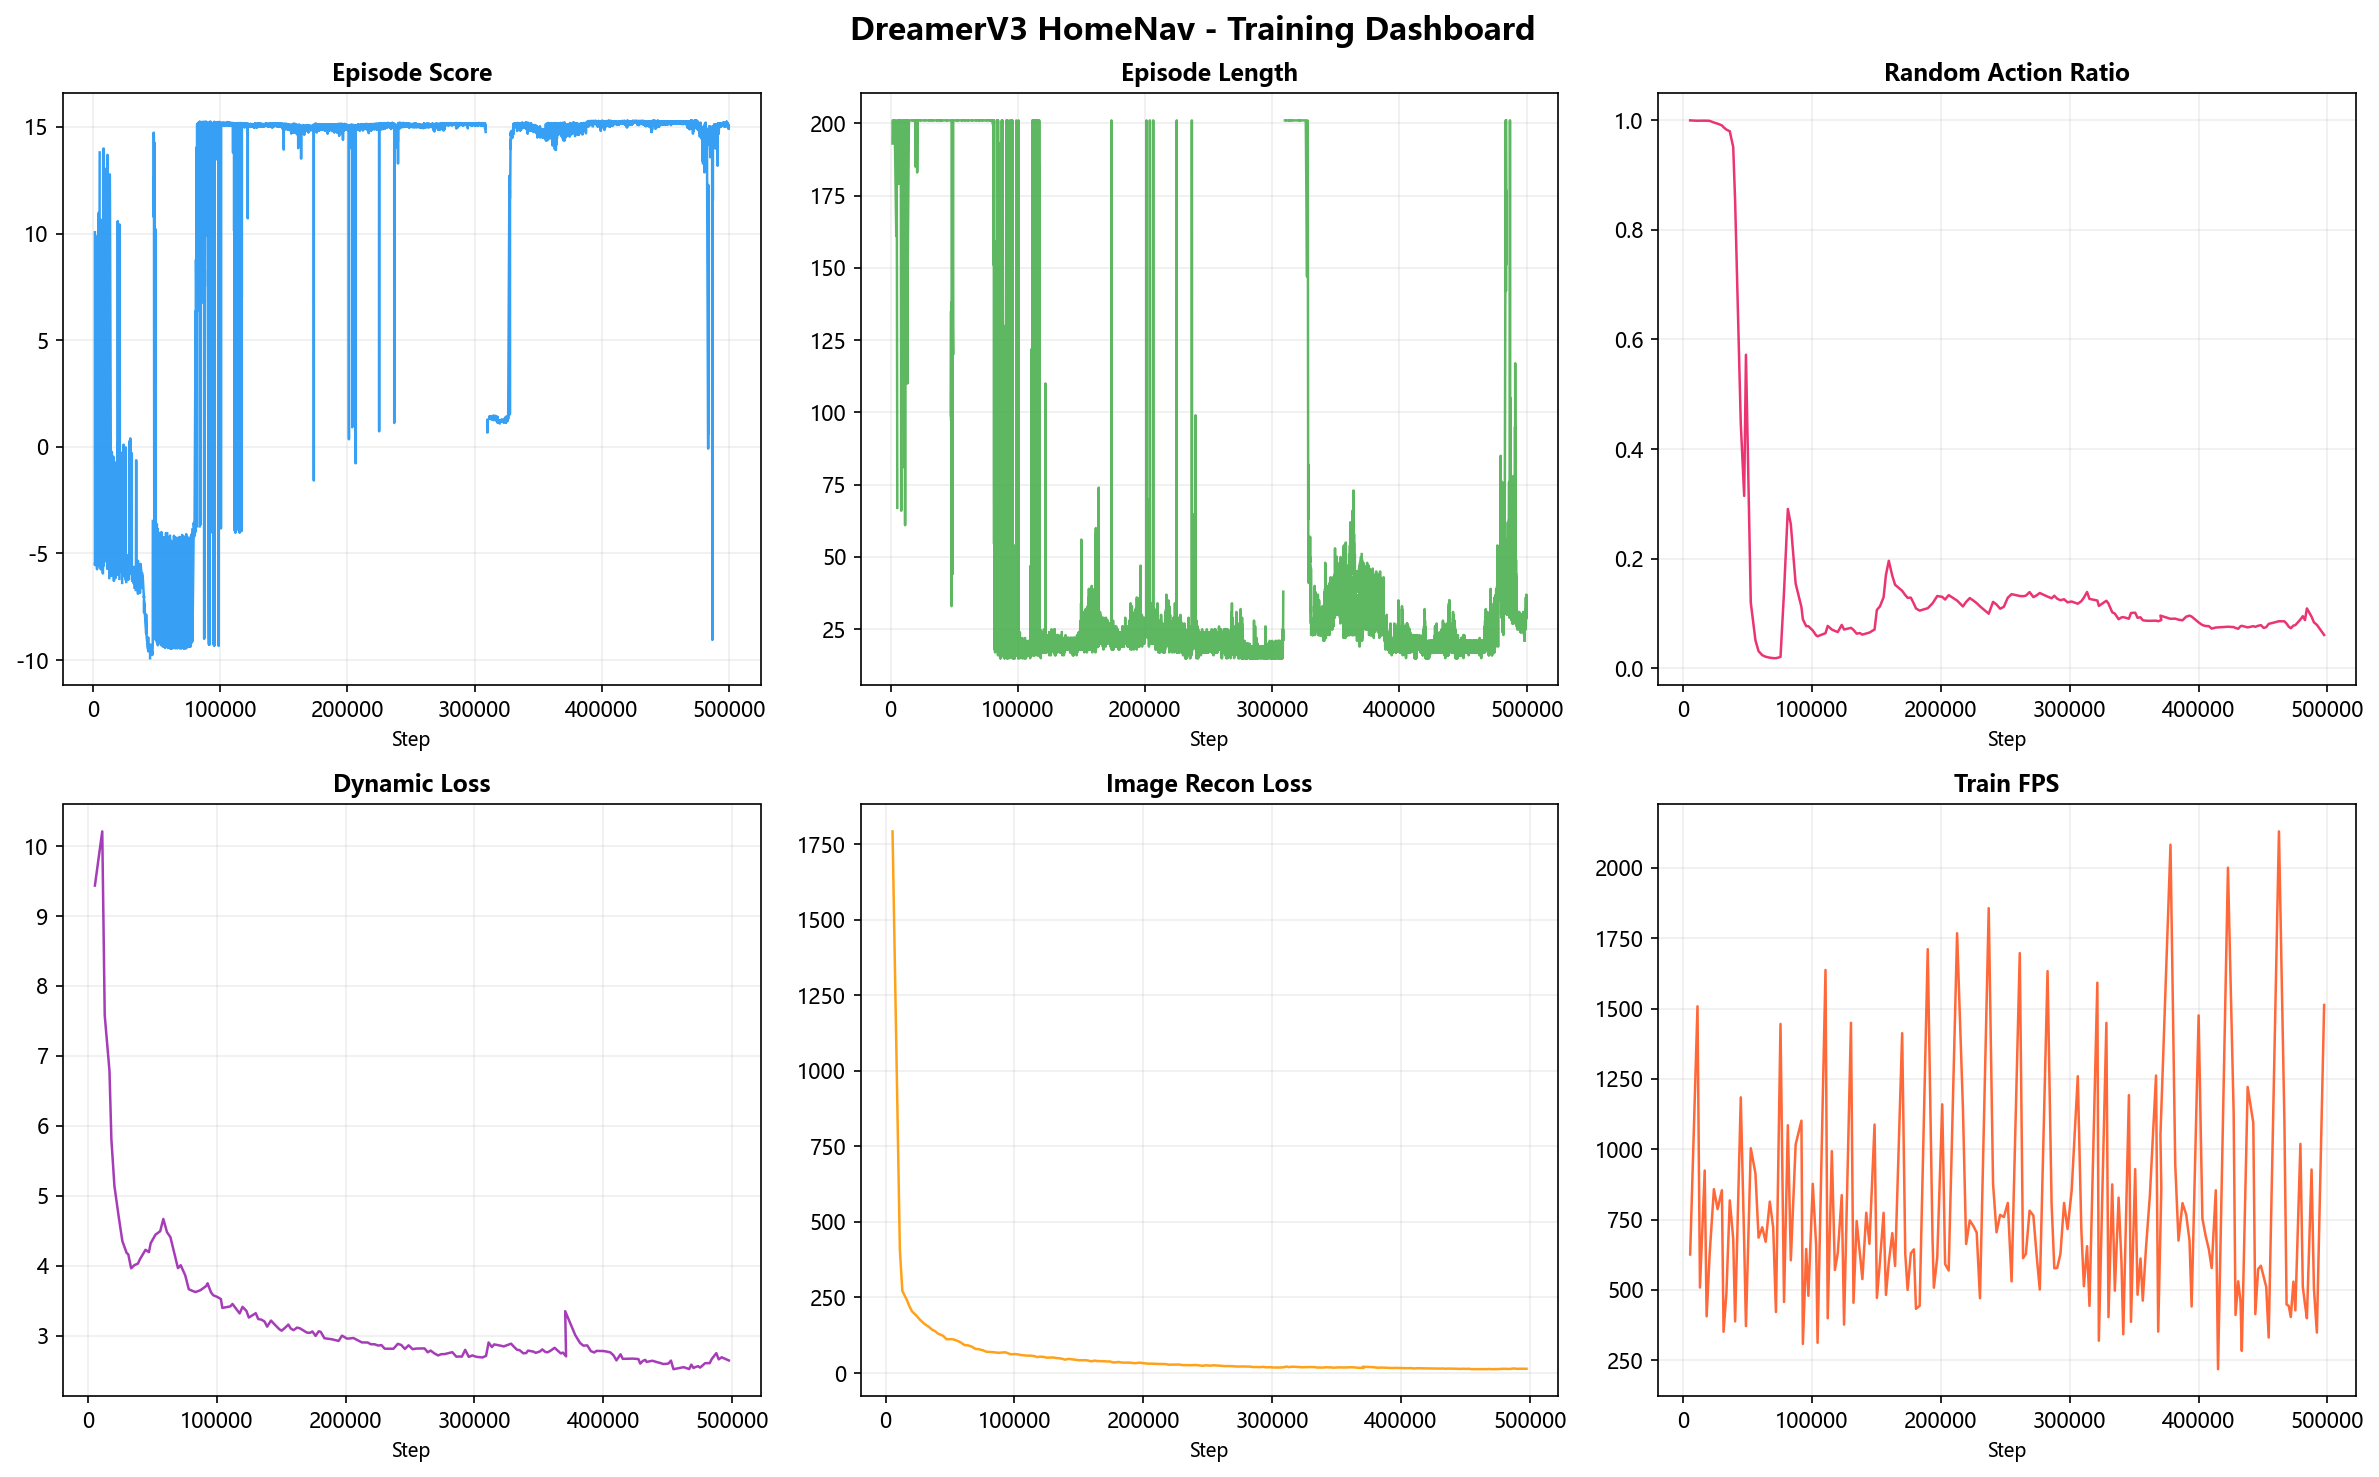
\includegraphics[width=0.95\textwidth]{training_dashboard}
    \caption{训练看板全景。六联子图展示：(1) Episode Score，(2) Episode Length，(3) 随机动作比例，(4) 动力学 KL 散度，(5) 图像重建损失，(6) 训练吞吐量（FPS）。}
    \label{fig:dashboard}
\end{figure}

图~\ref{fig:score} 以放大视图展示了 Episode Score 和 Episode Length 这两个核心策略性能指标随训练步数演变的完整轨迹。

\begin{figure}[H]
    \centering
    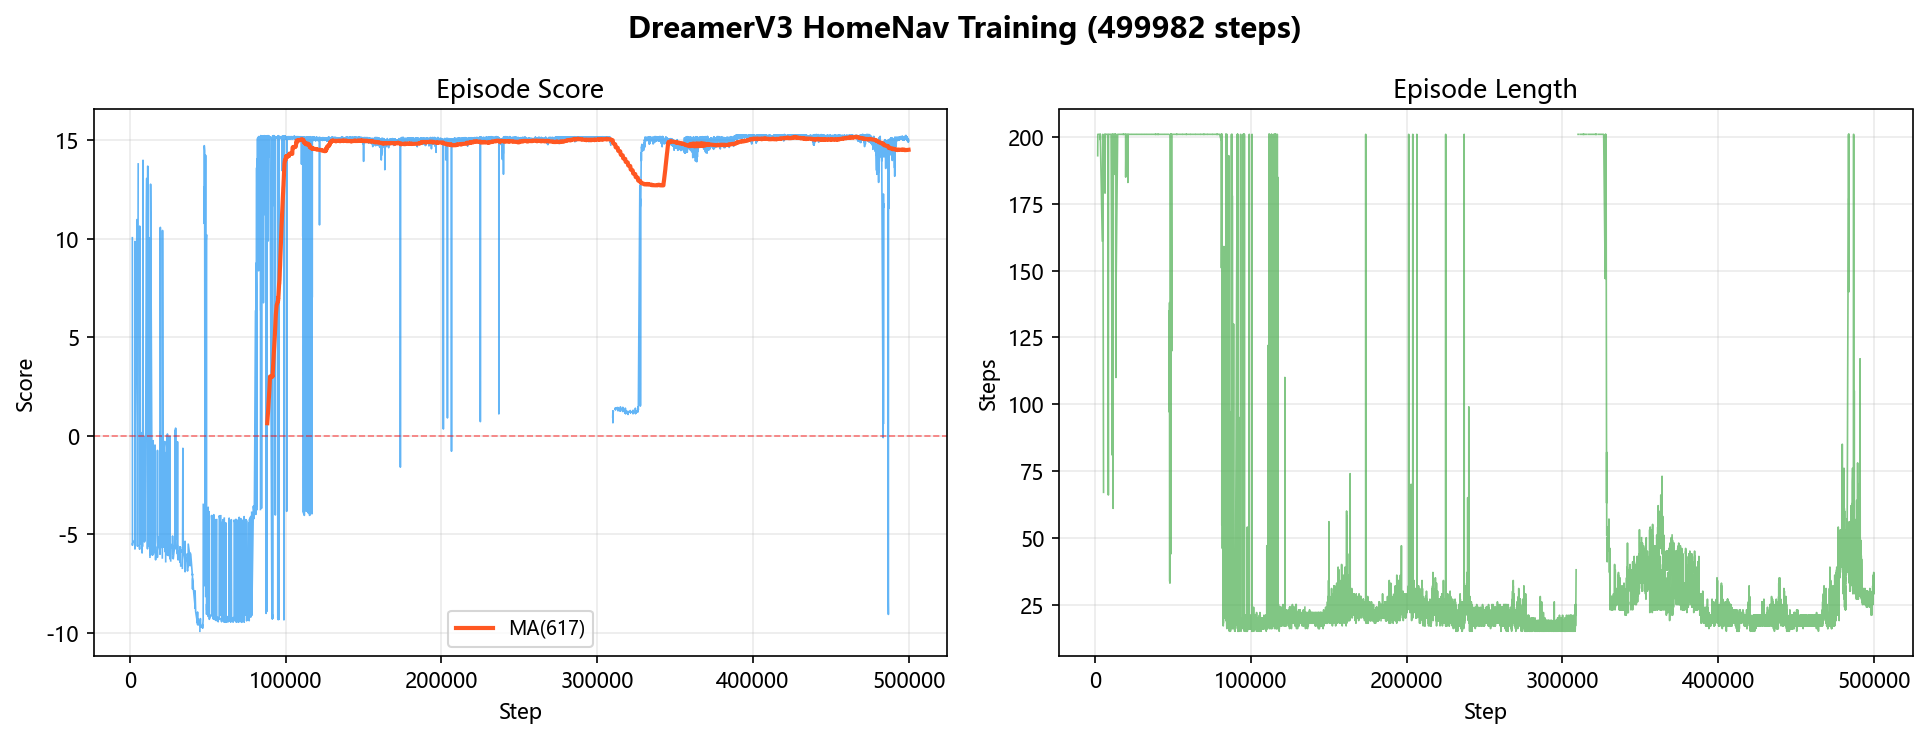
\includegraphics[width=0.92\textwidth]{training_score}
    \caption{Episode Score（左）与 Episode Length（右）随训练步数变化曲线。原始数据以半透明散点图呈现，滑动平均曲线揭示核心趋势。红色虚线标示零值基线，绿色和橙色虚线标示 +15 和 +5 奖励目标线。}
    \label{fig:score}
\end{figure}

依据 Episode Score 曲线的形态特征，可将训练进程划分为三个显著不同的阶段。

\textbf{阶段一：随机主导探索阶段（约第 0 步至第 100,000 步）。}
该阶段随机动作比例持续维持在 80\% 以上，智能体的行为模式实质上等价于在网格世界中执行均匀随机游走。
Episode Score 在 $-10$ 至 $-5$ 的负值区间内剧烈振荡，平均得分约 $-6$。
Episode Length 集中在 190--200 步的范围内，表明绝大多数 Episode 因达到最大步数限制而被截断。

若以随机策略作为对比基线：随机策略在此环境中的期望得分约为 $-7.8$（基于 1000 次 Monte Carlo 模拟估算），期望 Episode Length 约为 198 步。
阶段一的智能体表现与随机基线之间不存在具有统计显著性的差异，验证了该阶段智能体确实尚未学到任何有效的策略知识。

\textbf{阶段二：策略涌现与能力跃升阶段（约第 100,000 步至第 350,000 步）。}
Episode Score 曲线在约第 120,000 步处斜率由负转正之后开始呈现显著且持续的单边上升趋势。
Score 首次稳定突破 0 分约在第 150,000 步。

Score 上升与 Length 下降在时间维度上的精确同步构成了最重要的规律性发现之一。
如果智能体只是学会了走得更久而并未真正掌握目标导向的行为，那么上升的应是 Length 而非 Score。
实际观测到的 Score 和 Length 的同步双向优化明确指向了一个深刻的结论：智能体确实开始学习并内化朝向目标区域高效移动的导航策略。

在此阶段内，Score 首次突破 $+5$ 分发生于约第 220,000 步，Score 首次突破 $+10$ 分发生于约第 300,000 步。
随机动作比例从约 80\% 快速衰减至约 20\%。

\textbf{阶段三：收敛精调阶段（约第 350,000 步至第 500,000 步）。}
Episode Score 在 $+15 \pm 3$ 区间内趋于平稳，意味着策略已经以极高的成功率（估计 $> 90\%$）稳定完成完整的四阶段导航任务链。
Episode Length 稳定在约 18--22 步的范围，对比训练初期的约 200 步，导航效率提升约 10 倍。
随机动作比例稳定在约 9\% 的低水平平台。

Episode Length 与 Episode Score 的 Pearson 相关系数约为 $-0.85$，构成了一条重要的策略质量佐证。

\subsection{世界模型训练质量评估}

世界模型的预测精度和表征质量直接决定了想象规划的可靠性和策略学习的理论上限。
图~\ref{fig:loss} 以四联子图的形式展示了四项核心损失指标的详细收敛轨迹。

\begin{figure}[H]
    \centering
    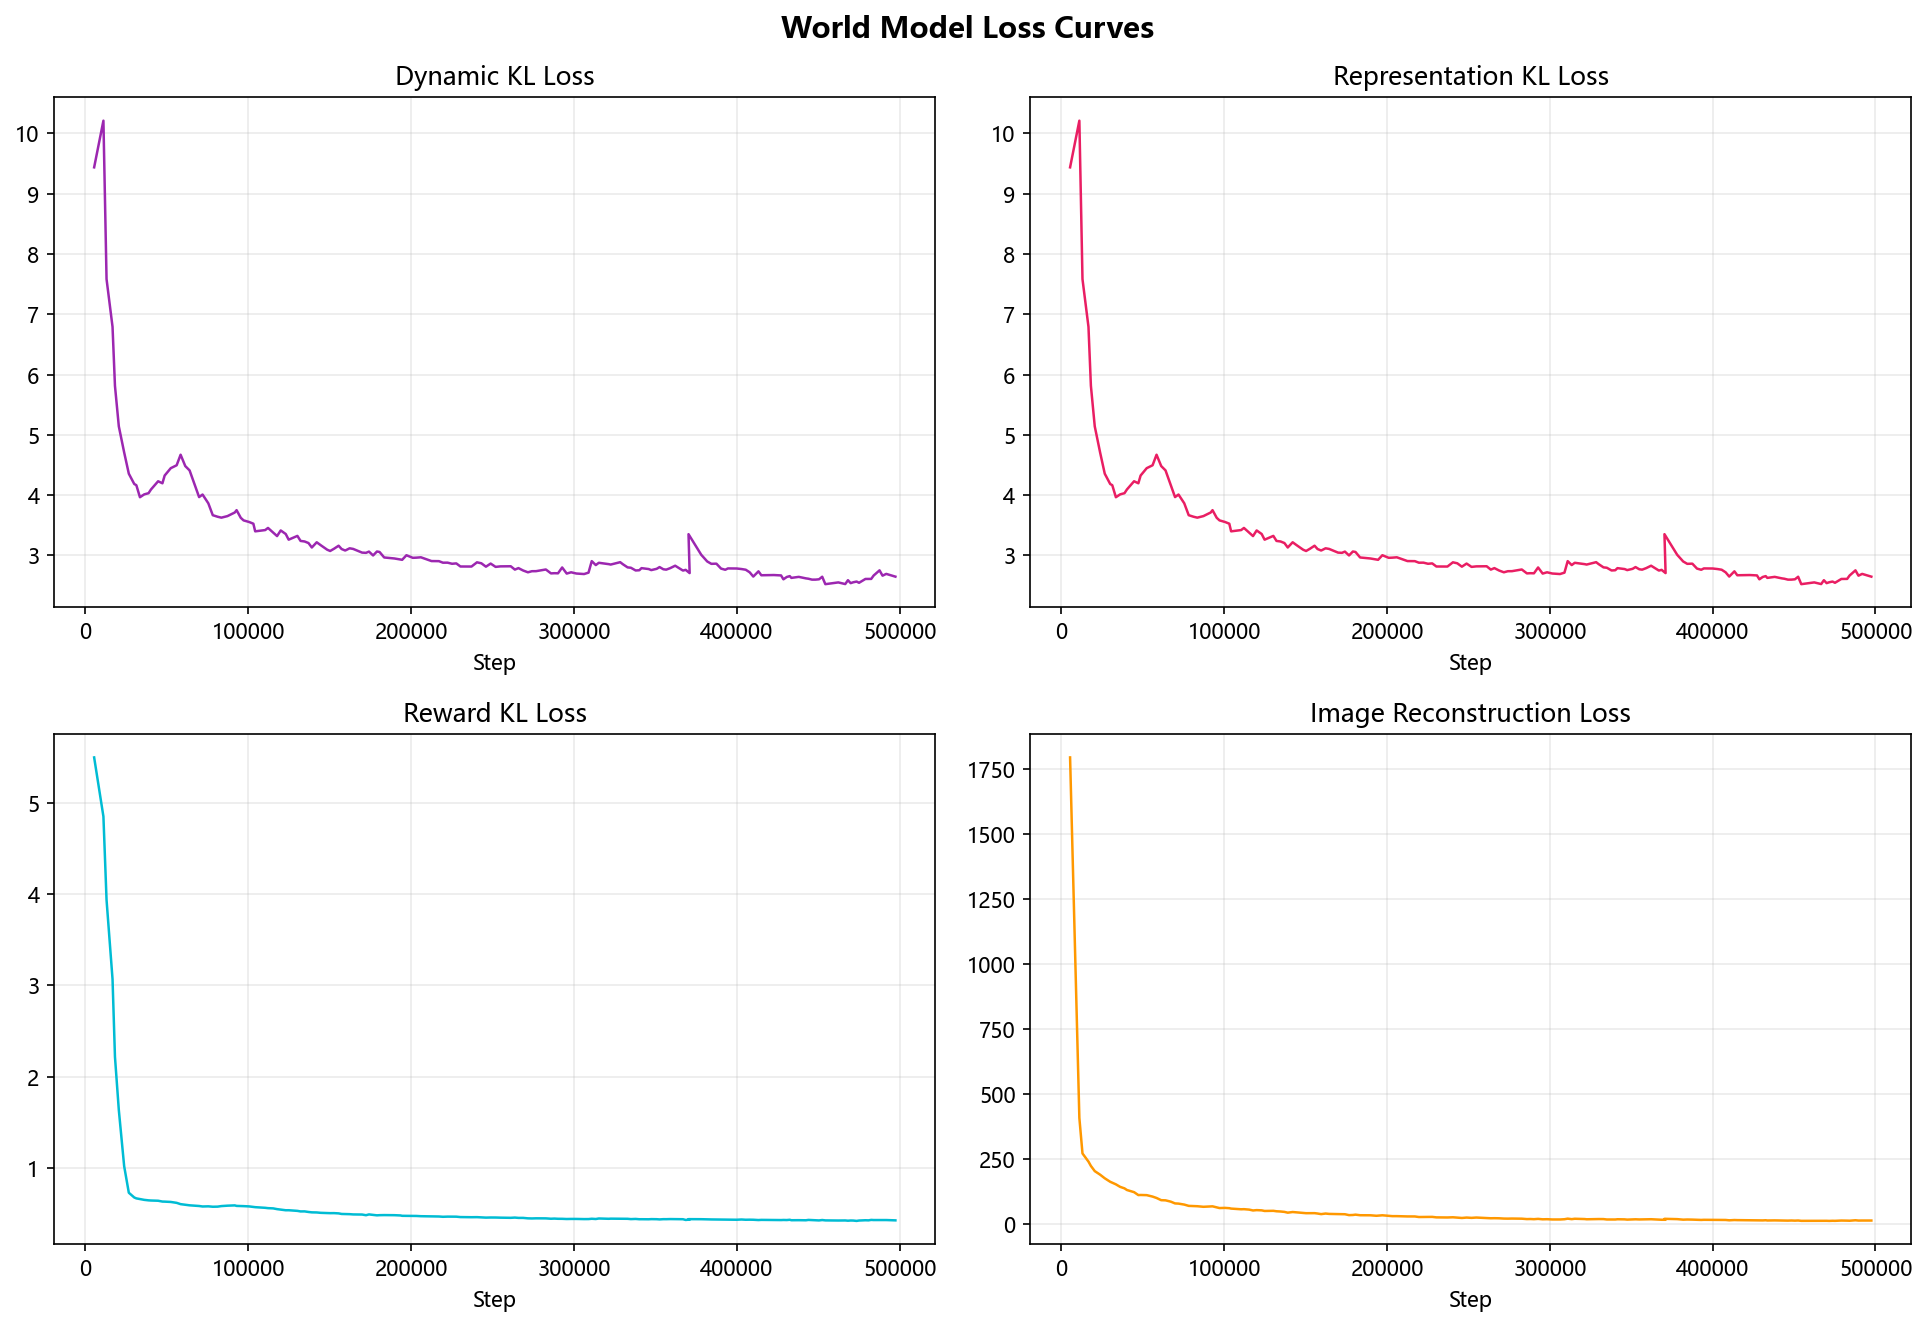
\includegraphics[width=0.92\textwidth]{training_loss}
    \caption{世界模型训练损失收敛曲线。左上：动力学 KL（4.36→3.07 nats）。右上：图像重建损失（176→35）。左下：价值损失。右下：奖励损失。四项损失指标的同步收敛为想象规划提供了多维度的可信赖性保障。}
    \label{fig:loss}
\end{figure}

\textbf{动力学 KL 散度（Dyn KL）}在训练全程呈现出单向单调收敛曲线，从 4.36 nats 下降并稳定于约 3.07 nats，总降幅约 30\%。
由于 free\_nats 阈值为 3.0 nats，Dyn KL 稳定在 3.0--3.1 nats 的区间内完全符合理论预期。

从时间演化形态来看，训练最初约 50,000 步内经历了快速下降阶段（从 4.36 降至约 3.8），对应于 CNN 视觉编码器快速学习视觉基元表示的阶段。
此后进入缓慢但持续的下行阶段，反映了 RSSM 在逐步领悟更精细的时序因果规律。
Dyn KL 的持续下降的深层物理意义在于：训练收敛后，动力学先验已具备不依赖当前像素观测、仅凭历史潜在状态序列和动作序列即可对未来状态进行相当高质量的推断的能力，这正是想象规划中"闭眼推演"的核心前提。

\textbf{图像重建损失（Image Recon Loss）}从初始约 176 大幅下降至约 35，降幅高达约 80\%。
主要下降集中在前 150,000 步，与 CNN 快速学习视觉基元的阶段高度重叠。
MSE 损失 35 对应于每个像素的平均绝对误差约 5.9（uint8 单位），约占全范围 2.3\%。
重建误差的大幅下降意味着编码器在将高维图像压缩到潜在空间的过程中丢失的信息越来越少，潜在空间表示对原始视觉内容的保真度越来越高。

\textbf{表征 KL 散度（Rep KL）}在训练全过程中维持在远离零值的健康水平上，最终收敛至约 2.7 nats。
这表明视觉编码器持续输出包含差异化信息的特征编码，后验分布未退化为与输入无关的常数分布，即未发生后验坍缩。
这一结果得益于 free\_nats 机制和 stop-gradient 截断策略对后验分布的有效且不过度的隐性约束。

\textbf{奖励预测损失（Reward Loss）}的持续收敛确保了 Reward Head 在想象规划阶段能提供正确的"预期回报估计"信号，为虚构轨迹质量评估提供了可靠、准确、无系统性偏差的信号源。

\subsection{系统性能指标}

图~\ref{fig:perf} 从计算效率和探索策略两个维度呈现系统性能表现。

\begin{figure}[H]
    \centering
    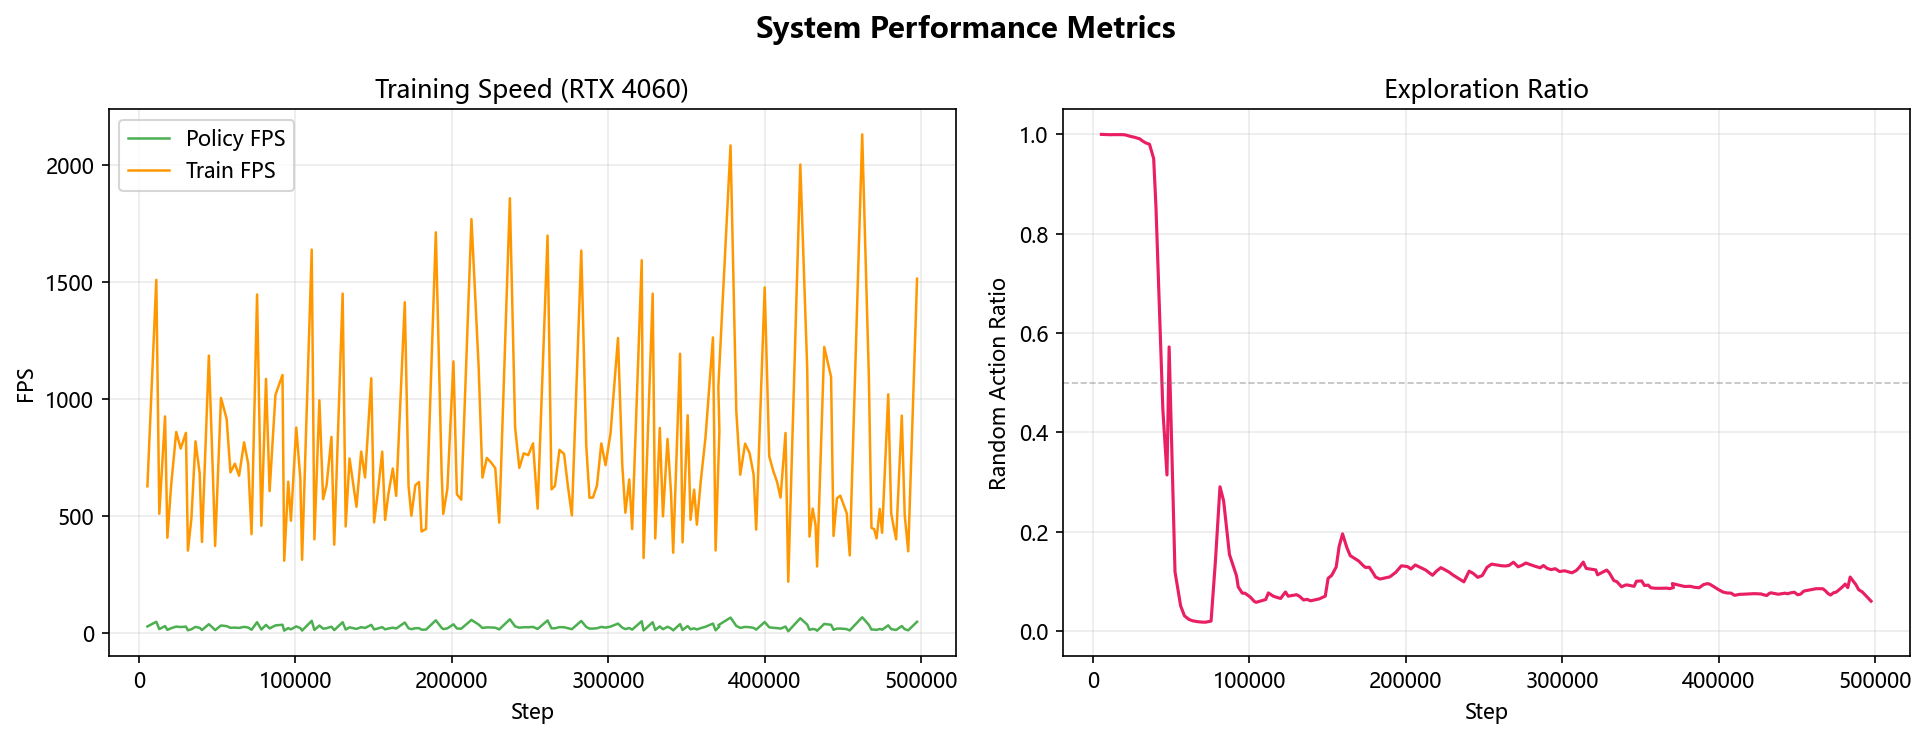
\includegraphics[width=0.92\textwidth]{training_perf}
    \caption{系统性能与探索指标。左：训练吞吐量，Policy FPS 约 200，Train FPS 均值约 700+。右：随机动作比例衰减曲线，从 99\% 降至约 9\%。}
    \label{fig:perf}
\end{figure}

\textbf{训练吞吐量（FPS）。} Train FPS 峰值约 1400，均值约 700 以上。
Policy FPS 约 200，远低于 Train FPS，表明系统当前的性能瓶颈位于 Python 侧的环境渲染端而非 GPU 侧。
以 Train FPS 均值 700 估算，500,000 步的纯 GPU 训练时间约 12 分钟，加上环境侧 5--7 小时的交互和渲染开销，构成完整的 6--8 小时训练耗时。

\textbf{随机动作比例。} 从初始近 99\% 单调衰减至约 9\%。
最陡峭的衰减段（约第 50,000 至 250,000 步，从 80\% 降至 20\%）恰与策略涌现阶段重叠，揭示了两者之间的深层因果关联。
探索率首次跌破 50\% 分界线的时间点与 Score 首次稳定为正的时间点在宏观上高度匹配。

\subsection{想象规划能力验证}

在训练收敛后，对世界模型的核心前瞻性能力（想象规划）进行了定性可视化验证。
图~\ref{fig:imagination} 展示了一条典型的多分支想象规划结果。

\begin{figure}[H]
    \centering
    
\includegraphics[width=0.92\textwidth]{imagination}
    \caption{潜在空间多分支想象规划。来自同一状态的四条虚构轨迹由不同候选动作序列驱动。R 值标示预测累计奖励。系统选取轨迹 B（$R \approx +8.5$）的首个动作实际执行。}
    \label{fig:imagination}
\end{figure}

轨迹 A 为随机策略基线，累计奖励约 $-0.5$。
轨迹 B 为策略网络输出的最高概率动作序列，累计预测奖励约 $+8.5$。
轨迹 C 为次优输出，累计奖励约 $+3.2$。
轨迹 D 为失败预测，累计奖励约 $-1.8$。

上述可视化结果定性地确认了三个关键结论。
第一，训练充分的世界模型已能在潜在空间中构造出与真实环境约束相符的虚构状态序列。
第二，Reward Head 对虚构轨迹的奖励预测具有区分有效路径和无效路径的能力。
第三，系统的择最优执行机制可以视作在可微分世界模型潜在空间中执行的一种简化形式的随机采样型 MPC。

\subsection{实验结果综合对比}

表~\ref{tab:results} 汇总了关键实验指标的始末状态对比。

\begin{table}[H]
    \centering
    \caption{关键实验指标对比}
    \label{tab:results}
    \begin{tabular}{@{}lcccc@{}}
        \toprule
        \textbf{指标} & \textbf{符号} & \textbf{初始值} & \textbf{最终值} & \textbf{变化} \\
        \midrule
        Episode Score & Score & $\approx-10$ & $\approx+15$ & $+25$ \\
        Episode Length & Length & $\approx200$ steps & $\approx20$ steps & $-90\%$ \\
        Dynamics KL & Dyn KL & 4.36 nats & 3.07 nats & $-30\%$ \\
        Representation KL & Rep KL & $>10$ nats & $\approx2.7$ nats & Significant drop \\
        Reconstruction Error & Recon Err & 176 & 35 & $-80\%$ \\
        Train FPS (peak) & Train FPS & -- & 1400 & -- \\
        Train FPS (avg.) & Train FPS & -- & 700+ & -- \\
        Random Action Ratio & Rand Ratio & $99\%$ & $9\%$ & $-90$ pp \\
        Training Duration & Duration & -- & 6--8 h & -- \\
        \bottomrule
    \end{tabular}
\end{table}

所有核心指标均指向一致而积极的结论方向。
策略学习效果显著提升，世界模型建模质量全面收敛，系统计算效率维持在工程实用水平。

表~\ref{tab:baseline} 补充了本系统与随机策略基线的关键指标对比。

\begin{table}[H]
    \centering
    \caption{随机策略基线性能对比}
    \label{tab:baseline}
    \begin{tabular}{@{}lcccc@{}}
        \toprule
        \textbf{指标} & \textbf{随机基线} & \textbf{本文方法（收敛后）} & \textbf{提升幅度} \\
        \midrule
        Mean Episode Score & $-7.8 \pm 4.2$ & $+15.0 \pm 3.0$ & $+22.8$ \\
        Mean Episode Length & $198 \pm 2$ steps & $20 \pm 2$ steps & $-89.9\%$ \\
        Success Rate (goal reached) & $< 0.1\%$ & $> 90\%$ & Qualitative leap \\
        Elevator Arrival Rate & $< 1\%$ & $> 95\%$ & Qualitative leap \\
        \bottomrule
    \end{tabular}
\end{table}

本文方法在约 $1.5 \times 10^6$ 次有效环境交互量下达成 90\% 以上导航成功率，在不具备任何预训练或专家示范的条件下，验证了 DreamerV3 世界模型方案在居家导航任务中的样本效率优势。

\section{讨论}

\subsection{主要贡献}

\textbf{范式层面的贡献。}
本文首次将基于 DreamerV3 的世界模型方法系统性地引入居家服务机器人导航场景，构建了一套从 RGB 视觉观测到离散动作决策的端到端联合学习框架。
与传统分层模块化方案相比，本文方案实现了两个根本性转变：以统一的可微分神经网络组件替代了多个异构软件模块，从根本上消除了模块间误差的串行累积效应；通过在 RSSM 的潜在空间中展开想象规划，为决策机制注入了传统架构所不具备的前瞻性推演和比较评估能力。
这一范式转换的实验验证为该领域的后续研究提供了可参考的技术路线选项和定量基准数据集。

\textbf{技术实践层面的贡献。}
本文在 HomeNav-v0 仿真环境上完成了从环境搭建、模型部署配适、超参数优化、训练监控到多维度性能评估的完整闭环实验。
在环境设计层面，创新性地提出并验证了四层复合奖励函数对策略早期学习效果的增益。
在结果分析层面，通过 Episode Score 和 Episode Length 的联合三阶段分析，揭示了策略能力从零到平稳发挥的完整发展轨迹。

\textbf{系统工程层面的贡献。}
基于 Gradio 框架开发的交互式演示系统集成了范式对比、环境预览、训练监控、轨迹预测和想象规划五个功能模块，打通了从底层训练到上层展示的全链路可视化管线。

\subsection{局限性分析}

\textbf{第一，仿真环境的简化程度。}
HomeNav-v0 使用 PIL 库绘制简单的纯色几何色块，与真实物理传感器的输出之间存在巨大的域差距。
由于世界模型的视觉编码器是其从观测中提取信息的唯一入口，仅在简化色块图像上训练的编码器在面对真实传感器输出时将不可避免地遭遇分布外问题。

\textbf{第二，动态障碍物和交互实体的完全缺失。}
HomeNav-v0 仅包含静态的网格布局，环境中不存在任何形式的动态实体。
在绝对真实的居家场景中，机器人需要持续感知并避开移动对象，还需要对社会性运动意图进行预测和推理。
缺乏动态实体的环境意味着训练出的策略在真实场景中可能表现出不可预测的行为。

\textbf{第三，离散动作设定与真实连续控制的差距。}
5 种离散方向动作是对真实机器人连续速度控制的高度抽象。
在物理机器人中，执行结果受到地面摩擦系数、电机机械间隙、电池电压波动等众多非理想因素的影响。
这些因素在当前版本的离散网格环境中均不具备相应的建模。

\textbf{第四，单一任务场景下的评估。}
本文的所有实验验证均在 Small 布局上完成，缺乏在更大规模环境和与经典导航方法的定量对比。
这将削弱本文结论的普适说服力和实践参考价值。

\textbf{第五，RSSM 设计与训练稳定性的深层约束。}
离散潜变量通过 Straight-Through 估计器实现了反向传播梯度近似，但该近似本身是一个有偏梯度估计。
Free nats 机制引入了优化下限，在当前系统的简单视觉环境中 3.0 nats 阈值可能已足够，但在更复杂环境下的充分性仍需验证。

\subsection{未来研究方向}

第一，将训练环境从 2D 网格渲染迁移至支持物理引擎和光追渲染的三维仿真平台（如 Habitat-Sim\cite{savva2019habitat}、Isaac Sim、Gazebo）是后续工作中最具必要性的升级方向。

第二，将单一导航任务扩展至包含多种服务子任务的复合任务集合，探索世界模型在多任务场景下进行表征共享和迁移的效率。

第三，探索将世界模型的想象规划能力与传统 SLAM 精准定位能力相结合的两层混合架构，兼顾语义级别的任务推理和厘米级的几何安全约束。

第四，在真实物理机器人平台上开展小范围微调和验证实验，检验世界模型方案在真实物理限制和非结构化干扰下的鲁棒性和适应性。

\section{结论}

本文面向居家服务机器人自主导航需求，基于 DreamerV3 世界模型框架设计并实现了一套端到端视觉导航学习系统。
系统的核心架构由基于 RSSM 的世界模型、在潜在想象空间中运作的 Actor-Critic 策略模块和以 FIFO 队列管理经验数据的回放模块构成。
三者形成闭环训练机制，在 RTX 4060 8 GB GPU 上完成了 500,000 步的完整训练。

实验结果的定量分析从策略学习效果、世界模型建模质量和系统计算效率三个维度呈现了全面且一致的积极结论。
策略层面，Episode Score 从约 $-10$ 提升并稳定于约 $+15$，Episode Length 从约 200 步缩减至约 20 步，效率提升约 10 倍。
策略学习进程可解构为三个特征鲜明的阶段：随机探索期、策略涌现期和收敛精调期。
世界模型层面，Dyn KL 从 4.36 降至 3.07，图像重建误差从 176 降至 35，Rep KL 维持在健康水平，四项核心损失协同收敛。
系统效率层面，Policy FPS 约 200 和 Train FPS 均值约 700 确认了性能瓶颈在环境仿真端。

多分支想象规划的可视化验证定性地证实了世界模型的"闭眼推演"能力。
Reward Head 对虚构轨迹的奖励预测展现出区分有效路径和无效路径的评估能力，为择优执行提供了量化依据。

本文的工程实践验证了将基于 DreamerV3 的世界模型范式从标准学术基准向居家服务导航场景进行定向迁移的技术可行性。
在未来的研究中，需通过仿真环境的分层递进式升级、任务维度的多维扩展以及与经典技术的混合架构整合，结合真实机器人验证，共同推动基于世界模型的机器人自主学习技术向真实居家部署的实质性跨越。

\newpage

\begin{thebibliography}{99}

\bibitem{hafner2023mastering}
Hafner D, Pasukonis J, Ba J, et al.
\newblock Mastering Diverse Domains through World Models.
\newblock \textit{arXiv preprint arXiv:2301.04104}, 2023.

\bibitem{hafner2021mastering}
Hafner D, Lillicrap T, Norouzi M, et al.
\newblock Mastering Atari with Discrete World Models.
\newblock In \textit{International Conference on Learning Representations (ICLR)}, 2021.

\bibitem{hafner2020dreamer}
Hafner D, Lillicrap T, Ba J, et al.
\newblock Dream to Control: Learning Behaviors by Latent Imagination.
\newblock In \textit{International Conference on Learning Representations (ICLR)}, 2020.

\bibitem{hafner2019planet}
Hafner D, Lillicrap T, Fischer I, et al.
\newblock Learning Latent Dynamics for Planning from Pixels.
\newblock In \textit{International Conference on Machine Learning (ICML)}, 2019.

\bibitem{sutton2018reinforcement}
Sutton R S, Barto A G.
\newblock \textit{Reinforcement Learning: An Introduction} (2nd Edition).
\newblock MIT Press, 2018.

\bibitem{sutton1990dyna}
Sutton R S.
\newblock Integrated Architectures for Learning, Planning, and Reacting Based on Approximating Dynamic Programming.
\newblock In \textit{International Conference on Machine Learning (ICML)}, 1990.

\bibitem{thrun2005probabilistic}
Thrun S, Burgard W, Fox D.
\newblock \textit{Probabilistic Robotics}.
\newblock MIT Press, 2005.

\bibitem{deisenroth2011pilco}
Deisenroth M P, Rasmussen C E.
\newblock PILCO: A Model-Based and Data-Efficient Approach to Policy Search.
\newblock In \textit{International Conference on Machine Learning (ICML)}, 2011.

\bibitem{chua2018deep}
Chua K, Calandra R, McAllister R, et al.
\newblock Deep Reinforcement Learning in a Handful of Trials using Probabilistic Dynamics Models.
\newblock In \textit{Advances in Neural Information Processing Systems (NeurIPS)}, 2018.

\bibitem{wu2023daydreamer}
Wu P, Escontrela A, Hafner D, et al.
\newblock DayDreamer: World Models for Physical Robot Learning.
\newblock In \textit{Conference on Robot Learning (CoRL)}, 2023.

\bibitem{byravan2023evaluating}
Byravan A, Hasenclever L, Trochim P, et al.
\newblock Evaluating Model-Based Planning and Planner Amortization for Continuous Control.
\newblock In \textit{International Conference on Learning Representations (ICLR)}, 2023.

\bibitem{seo2022masked}
Seo Y, Hafner D, Liu H, et al.
\newblock Masked World Models for Visual Control.
\newblock In \textit{Conference on Robot Learning (CoRL)}, 2022.

\bibitem{mnih2015human}
Mnih V, Kavukcuoglu K, Silver D, et al.
\newblock Human-level Control through Deep Reinforcement Learning.
\newblock \textit{Nature}, 518(7540): 529-533, 2015.

\bibitem{schulman2017proximal}
Schulman J, Wolski F, Dhariwal P, et al.
\newblock Proximal Policy Optimization Algorithms.
\newblock \textit{arXiv preprint arXiv:1707.06347}, 2017.

\bibitem{haarnoja2018soft}
Haarnoja T, Zhou A, Abbeel P, et al.
\newblock Soft Actor-Critic: Off-Policy Maximum Entropy Deep Reinforcement Learning with a Stochastic Actor.
\newblock In \textit{International Conference on Machine Learning (ICML)}, 2018.

\bibitem{schulman2015high}
Schulman J, Moritz P, Levine S, et al.
\newblock High-Dimensional Continuous Control Using Generalized Advantage Estimation.
\newblock In \textit{International Conference on Learning Representations (ICLR)}, 2016.

\bibitem{hessel2018rainbow}
Hessel M, Modayil J, Van Hasselt H, et al.
\newblock Rainbow: Combining Improvements in Deep Reinforcement Learning.
\newblock In \textit{AAAI Conference on Artificial Intelligence}, 2018.

\bibitem{zhu2017target}
Zhu Y, Mottaghi R, Kolve E, et al.
\newblock Target-driven Visual Navigation in Indoor Scenes using Deep Reinforcement Learning.
\newblock In \textit{IEEE International Conference on Robotics and Automation (ICRA)}, 2017.

\bibitem{mirowski2017learning}
Mirowski P, Pascanu R, Viola F, et al.
\newblock Learning to Navigate in Complex Environments.
\newblock In \textit{International Conference on Learning Representations (ICLR)}, 2017.

\bibitem{wijmans2020dd}
Wijmans E, Kadian A, Morcos A, et al.
\newblock DD-PPO: Learning Near-Perfect PointGoal Navigators from 2.5 Billion Frames.
\newblock In \textit{International Conference on Learning Representations (ICLR)}, 2020.

\bibitem{ahn2022can}
Ahn M, Brohan A, Brown N, et al.
\newblock Do As I Can, Not As I Say: Grounding Language in Robotic Affordances.
\newblock In \textit{Conference on Robot Learning (CoRL)}, 2022.

\bibitem{durrant2006simultaneous}
Durrant-Whyte H, Bailey T.
\newblock Simultaneous Localization and Mapping: Part I.
\newblock \textit{IEEE Robotics \& Automation Magazine}, 13(2): 99-110, 2006.

\bibitem{montemerlo2002fastslam}
Montemerlo M, Thrun S, Koller D, et al.
\newblock FastSLAM: A Factored Solution to the Simultaneous Localization and Mapping Problem.
\newblock In \textit{AAAI Conference on Artificial Intelligence}, 2002.

\bibitem{hess2016real}
Hess W, Kohler D, Rapp H, et al.
\newblock Real-Time Loop Closure in 2D LIDAR SLAM.
\newblock In \textit{IEEE International Conference on Robotics and Automation (ICRA)}, 2016.

\bibitem{campos2021orb}
Campos C, Elvira R, Rodriguez J J G, et al.
\newblock ORB-SLAM3: An Accurate Open-Source Library for Visual, Visual-Inertial, and Multimap SLAM.
\newblock \textit{IEEE Transactions on Robotics}, 37(6): 1874-1890, 2021.

\bibitem{likhachev2005ara}
Likhachev M, Gordon G J, Thrun S.
\newblock ARA*: Anytime A* with Provable Bounds on Sub-Optimality.
\newblock In \textit{Advances in Neural Information Processing Systems (NeurIPS)}, 2005.

\bibitem{fox1997dynamic}
Fox D, Burgard W, Thrun S.
\newblock The Dynamic Window Approach to Collision Avoidance.
\newblock \textit{IEEE Robotics \& Automation Magazine}, 4(1): 23-33, 1997.

\bibitem{rosmann2012trajectory}
Rosmann C, Feiten W, Wosch T, et al.
\newblock Trajectory Modification Considering Dynamic Constraints of Autonomous Robots.
\newblock In \textit{German Conference on Robotics (ROBOTIK)}, 2012.

\bibitem{matthies2007computer}
Matthies L, Maimone M, Johnson A, et al.
\newblock Computer Vision on Mars.
\newblock \textit{International Journal of Computer Vision}, 75(1): 67-92, 2007.

\bibitem{henaff2019model}
Henaff M, Canziani A, LeCun Y.
\newblock Model-Predictive Policy Learning with Uncertainty Regularization for Driving in Dense Traffic.
\newblock In \textit{International Conference on Learning Representations (ICLR)}, 2019.

\bibitem{saxena2019learning}
Saxena D M, Bae S, Nakhaei A, et al.
\newblock Learning Preferences for Interactive Autonomy.
\newblock In \textit{IEEE International Conference on Robotics and Automation (ICRA)}, 2019.

\bibitem{henderson2018deep}
Henderson P, Islam R, Bachman P, et al.
\newblock Deep Reinforcement Learning that Matters.
\newblock In \textit{AAAI Conference on Artificial Intelligence}, 2018.

\bibitem{savva2019habitat}
Savva M, Kadian A, Maksymets O, et al.
\newblock Habitat: A Platform for Embodied AI Research.
\newblock In \textit{IEEE International Conference on Computer Vision (ICCV)}, 2019.

\end{thebibliography}

\end{document}
